% main.tex
% header.tex
\documentclass[a4paper,11pt,twoside,ngerman,color]{book}
\usepackage[a4paper,left=3.5cm,right=2.5cm,bottom=3.5cm,top=3cm]{geometry}

\usepackage[german,english]{babel}

\usepackage[pdftex]{graphicx,color}
\usepackage{amsmath,amssymb,subfigure}

% Theorem-Umgebungen
\usepackage[amsmath,thmmarks]{ntheorem}

% Korrekte Darstellung der Umlaute
\usepackage[utf8]{inputenc}
\usepackage[T1]{fontenc}

% Algorithmen
\usepackage[plain,chapter]{algorithm}
\usepackage{algorithmic}

\usepackage{enumerate}

\usepackage{acronym}
\usepackage{listings}
\usepackage{color}
\lstdefinelanguage{Xtend}{
	morekeywords={cached,case,default,extension,false,JAVA,WORKFLOWSLOT,let,new,null,private,create,switch,this,true,reexport,around,if,then,else, def, val, var, private, class, static, return, as, instanceof, for, override, boolean,ENDFOR,FOR,ENDIF,IF},
	morekeywords=[3]{FAST, NORMAL, IN, PROVIDED},
	keywordstyle=[3]\color{eclipseBlue}\textsl,
	morekeywords=[4]{genDeclaration,genSuspension,genAction,genRegion,file,head,find},                        % <-- Your keywords here (w/ orange)
	keywordstyle=[4]\color{eclipseOrange},
    deletekeywords={scchart.},
	morecomment=[l]{//}, 
	morecomment=[s]{/*}{*/}, 
}

\definecolor{eclipseOrange}{RGB}{200,48,0}
\definecolor{eclipseBlue}{RGB}{0,0,172}
\definecolor{mygreen}{rgb}{0,0.6,0}
\definecolor{mygray}{rgb}{0.5,0.5,0.5}
\definecolor{mymauve}{rgb}{0.58,0,0.82}
\definecolor{compiler}{rgb}{0.53,0.12,0.47}
\lstset{ 
  backgroundcolor=\color{white},   % choose the background color; you must add \usepackage{color} or \usepackage{xcolor}; should come as last argument
  basicstyle=\footnotesize,        % the size of the fonts that are used for the code
  breakatwhitespace=false,         % sets if automatic breaks should only happen at whitespace
  breaklines=true,                 % sets automatic line breaking
  morecomment=[s][\color{red}]{/∗ }{ ∗/},
  captionpos=b,                    % sets the caption-position to bottom
  commentstyle=\color{mygreen},    % comment style
  deletekeywords={delete},            % if you want to delete keywords from the given language
  escapeinside={\%*}{*)},          % if you want to add LaTeX within your code
  extendedchars=true,              % lets you use non-ASCII characters; for 8-bits encodings only, does not work with UTF-8
  %firstnumber=1000,                % start line enumeration with line 1000
  frame=single,	                   % adds a frame around the code
  keepspaces=true,                 % keeps spaces in text, useful for keeping indentation of code (possibly needs columns=flexible)
  keywordstyle=\color{compiler},       % keyword style
  language=Octave,                 % the language of the code
  morekeywords={*,id,graphModel,container,node,edge,diagramExtension,style,containableElements,attr,extends,prime,this,EString,EBoolean,as,incomingEdges,outgoingEdges,position,appearance,lineWidth,lineStyle,background,foreground,font,BOLD,nodeStyle,roundedRectangle,size,corner,text,CENTER,TOP,value,rectangle,LEFT,MIDDLE,ellipse,edgeStyle,location,ARROW,movable,CIRCLE,decorator,points,appearanceProvider,polyline,polygon},            % if you want to add more keywords to the set
  morecomment=[s]{/*}{*/},
  morecomment=[l]{//},
  deletekeywords={delete,info},
  numbers=left,                    % where to put the line-numbers; possible values are (none, left, right)
  numbersep=5pt,                   % how far the line-numbers are from the code
  numberstyle=\tiny\color{mygray}, % the style that is used for the line-numbers
  rulecolor=\color{black},         % if not set, the frame-color may be changed on line-breaks within not-black text (e.g. comments (green here))
  showspaces=false,                % show spaces everywhere adding particular underscores; it overrides 'showstringspaces'
  showstringspaces=false,          % underline spaces within strings only
  showtabs=false,                  % show tabs within strings adding particular underscores
  stepnumber=2,                    % the step between two line-numbers. If it's 1, each line will be numbered
  stringstyle=\color{blue},     % string literal style
  tabsize=2,	                   % sets default tabsize to 2 spaces
  title=\lstname                   % show the filename of files included with \lstinputlisting; also try caption instead of title
}

% Bibtex deutsch
\usepackage{bibgerm}

% URLs
\usepackage{url}

% Caption Packet
\usepackage[margin=0pt,font=small,labelfont=bf]{caption}
% Gliederung einstellen
%\setcounter{secnumdepth}{5}
%\setcounter{tocdepth}{5}

% Theorem-Optionen %
\theoremseparator{.}
\theoremstyle{change}
\newtheorem{theorem}{Theorem}[section]
\newtheorem{satz}[theorem]{Satz}
\newtheorem{lemma}[theorem]{Lemma}
\newtheorem{korollar}[theorem]{Korollar}
\newtheorem{proposition}[theorem]{Proposition}
% Ohne Numerierung
\theoremstyle{nonumberplain}
\renewtheorem{theorem*}{Theorem}
\renewtheorem{satz*}{Satz}
\renewtheorem{lemma*}{Lemma}
\renewtheorem{korollar*}{Korollar}
\renewtheorem{proposition*}{Proposition}
% Definitionen mit \upshape
\theorembodyfont{\upshape}
\theoremstyle{change}
\newtheorem{definition}[theorem]{Definition}
\theoremstyle{nonumberplain}
\renewtheorem{definition*}{Definition}
% Kursive Schrift
\theoremheaderfont{\itshape}
\newtheorem{notation}{Notation}
\newtheorem{konvention}{Konvention}
\newtheorem{bezeichnung}{Bezeichnung}
\theoremsymbol{\ensuremath{\Box}}
\newtheorem{beweis}{Beweis}
\theoremsymbol{}
\theoremstyle{change}
\theoremheaderfont{\bfseries}
\newtheorem{bemerkung}[theorem]{Bemerkung}
\newtheorem{beobachtung}[theorem]{Beobachtung}
\newtheorem{beispiel}[theorem]{Beispiel}
\newtheorem{problem}{Problem}
\theoremstyle{nonumberplain}
\renewtheorem{bemerkung*}{Bemerkung}
\renewtheorem{beispiel*}{Beispiel}
\renewtheorem{problem*}{Problem}

% Algorithmen anpassen %
\renewcommand{\algorithmicrequire}{\textit{Eingabe:}}
\renewcommand{\algorithmicensure}{\textit{Ausgabe:}}
\floatname{algorithm}{Algorithmus}
\renewcommand{\listalgorithmname}{Algorithmenverzeichnis}
\renewcommand{\algorithmiccomment}[1]{\color{grau}{// #1}}

% Zeilenabstand einstellen %
\renewcommand{\baselinestretch}{1.25}
% Floating-Umgebungen anpassen %
\renewcommand{\topfraction}{0.9}
\renewcommand{\bottomfraction}{0.8}
% Abkuerzungen richtig formatieren %
\usepackage{xspace}
\newcommand{\vgl}{vgl.\@\xspace} 
\newcommand{\zB}{z.\nolinebreak[4]\hspace{0.125em}\nolinebreak[4]B.\@\xspace}
\newcommand{\bzw}{bzw.\@\xspace}
\newcommand{\dahe}{d.\nolinebreak[4]\hspace{0.125em}h.\nolinebreak[4]\@\xspace}
\newcommand{\etc}{etc.\@\xspace}
\newcommand{\evtl}{evtl.\@\xspace}
\newcommand{\ggf}{ggf.\@\xspace}
\newcommand{\bzgl}{bzgl.\@\xspace}
\newcommand{\so}{s.\nolinebreak[4]\hspace{0.125em}\nolinebreak[4]o.\@\xspace}
\newcommand{\iA}{i.\nolinebreak[4]\hspace{0.125em}\nolinebreak[4]A.\@\xspace}
\newcommand{\sa}{s.\nolinebreak[4]\hspace{0.125em}\nolinebreak[4]a.\@\xspace}
\newcommand{\su}{s.\nolinebreak[4]\hspace{0.125em}\nolinebreak[4]u.\@\xspace}
\newcommand{\ua}{u.\nolinebreak[4]\hspace{0.125em}\nolinebreak[4]a.\@\xspace}
\newcommand{\og}{o.\nolinebreak[4]\hspace{0.125em}\nolinebreak[4]g.\@\xspace}
\newcommand{\oBdA}{o.\nolinebreak[4]\hspace{0.125em}\nolinebreak[4]B.\nolinebreak[4]\hspace{0.125em}d.\nolinebreak[4]\hspace{0.125em}A.\@\xspace}
\newcommand{\OBdA}{O.\nolinebreak[4]\hspace{0.125em}\nolinebreak[4]B.\nolinebreak[4]\hspace{0.125em}d.\nolinebreak[4]\hspace{0.125em}A.\@\xspace}

% Leere Seite ohne Seitennummer, naechste Seite rechts
\newcommand{\blankpage}{
 \clearpage{\pagestyle{empty}\cleardoublepage}
}

% Keine einzelnen Zeilen beim Anfang eines Abschnitts (Schusterjungen)
\clubpenalty = 10000
% Keine einzelnen Zeilen am Ende eines Abschnitts (Hurenkinder)
\widowpenalty = 10000 \displaywidowpenalty = 10000
% EOF

\begin{document}

\selectlanguage{english}
\begin{titlepage}
\definecolor{TUGreen}{rgb}{0.517,0.721,0.094}
\vspace*{-2cm}
\newlength{\links}
\setlength{\links}{-1.5cm}
\sffamily
\hspace*{\links}
\begin{minipage}{12.5cm}

\includegraphics[width=8cm]{bilder/tud_logo_rgb}
%\hspace*{-0.25cm} \textbf{TECHNISCHE UNIVERSIT"AT DORTMUND}\\
%\hspace*{-1.2cm} \rule{5mm}{5mm} \hspace*{0.1cm} FACHBEREICH INFORMATIK\\
\end{minipage}

\vspace*{4cm}

\hspace*{\links}
\hspace*{-0.2cm}
\begin{minipage}{9cm}
\large
\begin{center}
{\Large Bachelor Thesis} \\
\vspace*{1cm}
\textbf{A Graph Language for Sequentially Constructive Statecharts} \\
\vspace*{1cm}
Kristopher Tom Kettler\\
% \vspace*{1cm}
October 2023
\end{center}
\end{minipage}
\normalsize
\vspace*{5.5cm}

% \hspace*{\links}

\vspace*{2.1cm}

\hspace*{\links}
\begin{minipage}[b]{5cm}
% \normalsize
\raggedright
Supervisors: \\
%Name des Erstgutachters \\
Prof. Dr. Bernhard Steffen \\
%Name des Zweitgutachters \\
Dr. Steven Smyth \\
\end{minipage}

\vspace*{2.5cm}
\hspace*{\links}
\begin{minipage}[b]{8cm}
% \normalsize
\raggedright
TU Dortmund University \\
Faculty of Computer Science\\
Chair of Programming Systems (LS V)\\
http://ls5-www.cs.tu-dortmund.de
\end{minipage}
%%%%%%%%%%%%%%%%%%%%%%%%%%%%%%%%%%%%%%%%%%%%%%%%%%
% bei Kooperation mit anderen Lehrstuehlen,
% sonst weglassen
%\begin{minipage}[b]{8cm}
% \normalsize
%\raggedleft
%In Kooperation mit:\\
%Fakult"atsname\\
%Lehrstuhl-/Institutsbezeichnung
%\end{minipage}
%%%%%%%%%%%%%%%%%%%%%%%%%%%%%%%%%%%%%%%%%%%%%%%%%%

\end{titlepage}

\blankpage
\pagenumbering{roman}
\tableofcontents
\cleardoublepage
\pagenumbering{arabic}

% Kapitel
\chapter*{Abstract}
In the field of model-driven software development, domain-specific languages can make an important contribution to the development of software systems. Nevertheless, their use is not widespread because the development of domain-specific tools is often considered complex and tedious. To show that the development of such tools can also be made possible with relatively little effort, the development process of such a tool is shown in this context. For the development, the \textsc{Cinco} Meta Tooling Suite is used, whose main feature is the full generation of graph-based modeling tools. SCCharts, a visual modeling language for the specification of safety-critical reactive systems, serves as a representative for a domain-specific graphical modeling language for which the tool is developed.


% einleitung.tex
\chapter{Introduction}
The increasing complexity of software systems poses new challenges for software developers. As a result, the use of modeling languages to develop such systems has grown in popularity, helping developers to gain a better understanding of the system. In addition, code generators are often part of such tools, which generate executable code from the designed model that can be integrated into applications. In general, they help to increase the efficiency of the development process. Starting with textual languages such as VHDL for describing hardware or HTML markup language for developing web pages, to graphical modeling languages such as the well known UML, the model-based approach runs through every area of software development. Basically, a distinction is made between general-purpose modeling languages (GPMLs) and domain-specific languages (DSLs). The latter are mostly textual and require Language Workbenches, frameworks that support the development of according editors and tools for DSLs. Thereby, it provides similar features as modern Integrated Development Environments (IDEs). In addition, metamodeling frameworks such as the Eclipse Modeling Framework (EMF) or JetBrains Meta Programming System support the development of editors for DSLs.~\cite{Lybecait.2018}~\cite{Naujokat.2018}

However, the development of complicated domain-specific tools has often proved to be complex and laboriously. Also, most metamodeling frameworks focus on textual modeling languages, including those mentioned above, so support for graphical languages is rather sparse. For these reasons, the \textsc{Cinco} Meta Tooling Suite (\textsc{Cinco}) was developed. It offers a solution for the creation of graph-based modeling tools. Furthermore, it follows a simplicity-oriented approach, which means that universality is limited in favour of simplicity. The core feature of \textsc{Cinco} is the full generation of these domain-specific graphical modeling tools from meta-level specifications and models. This is a significant advantage over other approaches that only support semi-automatic generation of graphical editors from high-level specifications, and where the generated code still needs to be adapted before the editor can be executed.~\cite{Lybecait.2018}~\cite{Naujokat.2018}

\section{Motivation}
Although DSLs are often seen as a means to empower domain experts to create software systems on their own and thus replace programmers, this goal has not yet been achieved. However, it is already possible today for domain experts to understand and verify code written by developers. Nevertheless, DSLs seem to be less popular than GPMLs, of which there are many more variations. Naujokat et al.~\cite{Lybecait.2018} suggest that this is because people consider the complex development of DSL tools to be too complicated and elaborate, and therefore not worthwhile. This observation is the motivation for this bachelor thesis. With \textsc{Cinco} a solution has now been created that facilitates the creation of editors for graphical domain-specific languages by trading generality for simplicity. If it could be shown how easy it is to create a DSL tool using \textsc{Cinco}, this might convince more people to use DSLs and perhaps get one step closer to the vision of empowering domain experts to create their systems themselves with DSL tools.

\section{Problem Statement}
The central issue addressed in this bachelor thesis is the low popularity of DSLs, primarily attributed to the perceived complexity associated with the development of DSL tools. The complexity involved in creating DSL tools often makes it seem unworthy of the investment, leading to a preference for more GPMLs. Consequently, there is a need to investigate and demonstrate how \textsc{Cinco}, a tool that prioritizes simplicity in creating graphical DSL editors, can facilitate the development of such DSL tools. The SCCharts language~\cite{Hanxleden.2014}, a visual modeling language designed for specifying safety-critical reactive systems, was chosen as example of a graphical DSL for which the editor development process is shown.

Using this development process as an example, it should be shown that the development of DSL tools does not have to be tedious and complex, which should contribute to solving the problem of the low use of DSLs. To this purpose, the editor must provide some functionalities to support the development of SCCharts, so that it can be considered as a useful tool for the application of DSL tools. On the one hand, it should be possible to create and extend SCChart models. Potential users must be able to read the created models correctly. The visual syntax of the model created in the editor should therefore be as similar as possible to that of SCCharts. In addition, it should not be possible to create incorrect models or it should be indicated to the user if there are errors in the model. The user interface should be as user-friendly as possible so that users who are not programmers can also use the tool. Finally, the editor should be able to generate code from the created model that can be integrated into software systems. 

\section{Structure}
Chapter \ref{chapter_Foundations} presents the foundations of model-driven software development (Sect. \ref{Model-Driven Software Development}), which are essential for understanding the editor's development process, and introduces the SCCharts language (Sect. \ref{Sequentially_Constructive_Statecharts}), necessary for implementing the editor based on it. In Chapter \ref{Related_Work}, related work is addressed. Subsequently, Chapter \ref{Frameworks_and_Tools} deals with the tools and frameworks that were ultimately used to create the editor for SCCharts. The core of this bachelor thesis, the conception and implementation of the graphical DSL tool for SCCharts, is presented in Chapter \ref{Concept_and_Implementation_of_the_Graph_Language}. First, requirements for the SCCharts tool are defined (Sect. \ref{Requirements}). The data structure is then designed and the Meta Graph Language of the editor is implemented based on it. Then the Style Graph Language is adapted, which specifies the visual syntax of SCCharts components in the editor. Next, the user interface and the model validation are implemented. Finally, the code generator is realised in this Chapter. After the editor has been designed and implemented, it is evaluated in Chapter \ref{Evaluation_of_the_Model_Editor}. Finally, in Chapter \ref{Conclusion} a summary with conclusions is presented.


\chapter{Foundations}\label{chapter_Foundations}
This chapter provides conceptual foundations that are essential for understanding the development process of the editor. First, the basics of model-driven software development (MDSD) important in this context are presented, followed by an exploration of the SCCharts language.
\section{Model-Driven Software Development}\label{Model-Driven Software Development}
Before clarifying what exactly MDSD is, the term model must be defined more precisely.

\subsection{Model}
Generally a model can be said to serve as a simplified or partial representation of real entities, designed to emphasise essential information or features while omitting less important details. Models are used in many fields, from science to business, and serve as valuable tools to understand, analyse and communicate complicated phenomena or processes. In the realm of software engineering, models assume diverse roles, spanning from describing systems or the specification of requirements to the generation of configuration files or executable code based on the information encapsulated within these models.~\cite{Brambilla.2017}

\subsection{Goals of Model-Driven Software Development}
First of all, it should be clarified what is meant by MDSD. According to Brambilla et al.~\cite{Brambilla.2017}, MDSD "is a development paradigm that uses models as the primary artifact of the development process. Usually, in [MDSD] the implementation is (semi)automatically generated from the models." The aim is to use models as development artefacts and to use abstraction to hide the unimportant details and highlight the important ones. In addition, it tries to automate as much of the development process as possible. This can start with the definition of requirements and reach up to the final developed software system.

\subsection{Modeling Language}
Modeling languages are an important part in the MDSD. They serve as a mechanism through which designers can articulate both the structure and behavior of their systems, utilizing either graphical or textual representations. Designers are required to adhere to the specific syntax defined by the modeling language they are using. There are two primary classes of modeling languages: GPMLs and DSLs. DSLs are modeling languages designed for a specific domain or area of application. This specialization ease the process of creating models within that particular domain. Conversely, GPMLs can be applied to a wide range of applications but lack the tailored focus found in DSLs.~\cite{Brambilla.2017}

\subsection{Metamodeling}
The term metamodeling describes a concept for creating models from models. The model that is used to create another model is called a metamodel. Thus, a metamodel is essentially a model that describes the structure and semantic rules for a particular class of models. It is used to define the syntax and semantics of a modeling language and to ensure that models created in that language conform to the defined rules. 

A suitable example for this can be seen in Fig. \ref{fig:Meta-Modeling}. When describing real objects through models, the model level M1 defines the syntax and semantics of the level below it, M0. The same applies to the model level in relation to the metamodel level M2. For the metamodel level M2, once again, the syntax and semantics can be defined in the level above it, the meta-metamodel level. This process could continue indefinitely, so that starting from the meta-metamodel level, each subsequent meta-metamodel instance refers to another meta-metamodel instance.~\cite{Brambilla.2017}
\begin{figure}[h!]
\centering
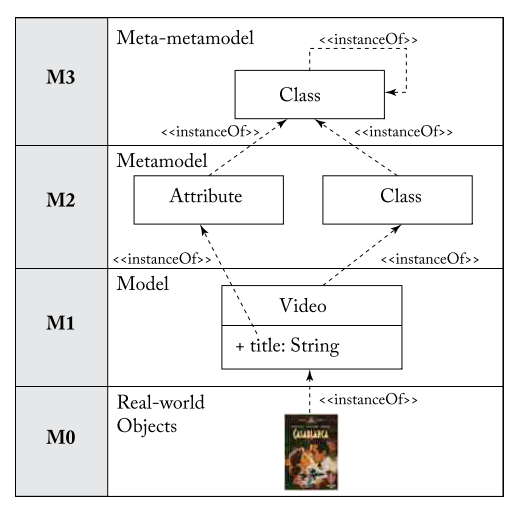
\includegraphics[width=0.7\textwidth]{bilder/Meta-Modeling.png}
\caption{Models, metamodels, and meta-metamodels (from~\cite{Brambilla.2017})}
\label{fig:Meta-Modeling}
\end{figure} 

This example can also be mapped to the creation of a DSL tool for SCCharts. In M3 is the \textsc{Cinco} meta tool with which a DSL tool for SCCharts is to be created (layer M2). This can then be used to create SCCharts models (M1) that represent a SCChart of the SCCharts language (M0).

\section{Sequentially Constructive Statecharts} \label{Sequentially_Constructive_Statecharts}
The visual modeling language SCCharts, which is based on Harel's Statecharts~\cite{Harel.1987}, was designed for safety-critical applications and aim for easy adaptation. It utilize the visual syntax from Charles André's SyncCharts~\cite{andre.} and provides deterministic concurrency based on a synchronous Model of Computation. 

To gain a better understanding of the different elements of the SCCharts syntax, Fig \ref{fig:SCChart-Overview} is helpful. The upper part of depicts the Core-SCCharts, which include concurrency and hierarchy as essential features of Statecharts. While the lower part contains elements of the Extended SCCharts. It should be noted that each advanced feature can be expressed as one or more core features, but the use of advanced features reduces the complexity of the diagram and therefore improves clarity.~\cite{Hanxleden.2014} The components are explained in more detail below.

\begin{figure}[h!]
\centering
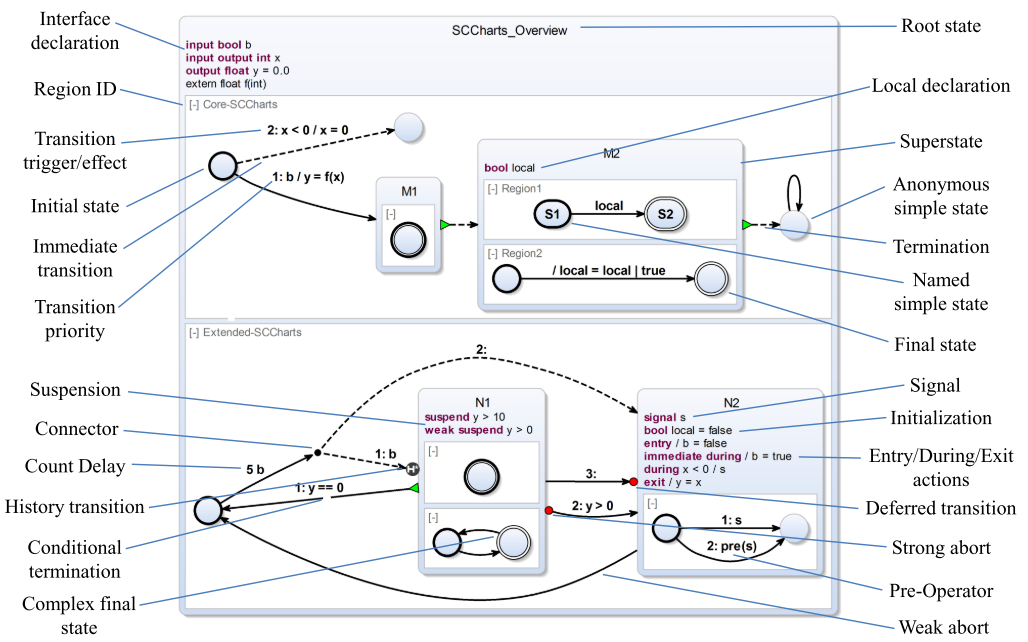
\includegraphics[width=1.0\textwidth]{bilder/SCChart-Overview.png}
\caption{SCCharts-Overview (from~\cite{Hanxleden.2014})}
\label{fig:SCChart-Overview}
\end{figure} 

\subsection{States and SuperStates}
States are a fundamental part of SCCharts. A distinction is made between simple states and states with internal behaviour, so-called superstates. Both types of states can function as initial states (thick border), final states (double border) or initial final states (thick border and double border). Each SCChart also has exactly one root state that behaves like a superstate and in which all behaviour of the SCChart is defined. Additionally, there are connectors (large black dot), which are essentially simple states with the purpose of connecting multiple states through outgoing and incoming edges.
\subsection{Transitions}
Another basic component is transitions. Each transition has a source state and a target state. Transitions can have a label with the syntax \textit{[p:] [t] [/ a]}, where p stands for priority, t for trigger and a for action. The trigger is a side-effect-free boolean expression and the action is an assignment of any data type. A state is said to be active when the SCChart is in that particular state. If the source state of a transition is active and the trigger becomes true, the target state is active. The transition can be immediate (dashed transition) or delayed. Immediate means that the state becomes active on the same tick (stimulus), while delayed means that the state becomes active on the next tick. Transitions are delayed by default to avoid causality problems. The priority is used to check the trigger in ascending order, so that if there are, for example, two transitions with true triggers, the one with the higher priority is used.~\cite{Motika.2017}
\subsection{Declarations}
Declarations of variables can be made at the top of any superstate, including root states. These variables can be inputs, which are read from the environment, or outputs, which are written to the environment. Additionally, they can also be input output variables or local variables, which are used only internally. The data types for these variables can include boolean, integer, float, and string. Local variables can also be uninitialized or pre-assigned, and their values persist even when, for example, the superstate where they are defined is exited. Furthermore, there are signals used for communication with the environment and among the components of the SCChart. Pure signals are interpreted as boolean values and are true when present and false when absent. In contrast, valued signals carry a typed value in addition to their presence status. Lastly, declarations can be marked as constant, which means that the value cannot be changed after initialization.~\cite{Motika.2017}
\subsection{Hierarchy and Concurrency}
Superstates, including the root state, have inner behavior, which includes one or several concurrent regions (represented by white boxes). Each region conceptually corresponds to a thread, and each region must contain an initial state. If a final state is entered within a region, that region terminates. Termination transitions (green triangle at the source state) can originate from superstates and are taken when all regions within the superstate are in final states. These transitions are typically unconditional, and superstates usually have only one of them. If there are multiple termination transitions, the one with the highest priority is taken.~\cite{Motika.2017}

\subsection{Actions and Suspensions}

Actions and suspensions are specified beneath the declarations of superstates. There are four distinct types of actions that influence the behavior of the associated superstate. These actions have an effect and may include an optional condition. Entry and exit actions are executed when entering or exiting the superstate, either when they have no condition or when their optional condition evaluates to true. Additionally, there are during and immediate during actions, which are executed if the superstate they are associated with is active and they either have no condition or a condition that evaluates to true. Depending on their type, they may be executed with a delay or immediately.~\cite{Motika.2017}

Suspensions suppress the inner behavior of a superstate, if their trigger is evaluated to true. Their also four different types. Immediate and delayed suspensions are self-explanatory. Weak suspensions and immediate weak suspensions allows immediate inner behavior of a suspensions state but the weakly suspended state remains in the exact same internal states.~\cite{Motika.2017}

\subsection{Complex Transitions}
Beyond the simple transitions described initially, there are additional transitions that have effects upon entering or exiting superstates. One of these is history transition (H at the target state), which allows the execution to continue in the state that was active when the superstate was left. Shallow history applies only to the top level of the superstate, while deep history (H with *) reaches into the deeper levels as well. Furthermore, there are deferred transitions (red dot at the target state), which preempt all immediate behavior in the target state. Finally, there are strong abort transitions (red dot at the source state). Unlike weak aborts (default transitions), which allow the inner behavior of superstates to continue during the tick, strong aborts terminate them directly.
Additionally, transitions can have a count delay. This means that the condition must be true for a specific number of ticks before the transition is triggered.~\cite{Motika.2017}

\subsection{References}
Another feature of SCCharts is their ability to reference each other. To achieve this, the corresponding inputs and outputs of the referenced SCChart must be assigned variables of the appropriate type. These references then become superstates within the inner behavior of the referenced SCChart. Figure \ref{fig:Beep-Reference} illustrates an example of such a reference. Here, Beep is referenced as a superstate within the region of Root. In this case, the input boolean second from Root is assigned to the input second of Beep, and the output boolean speaker from Root is assigned to the output boolean beep of Beep.
\begin{figure}[h!]
\centering
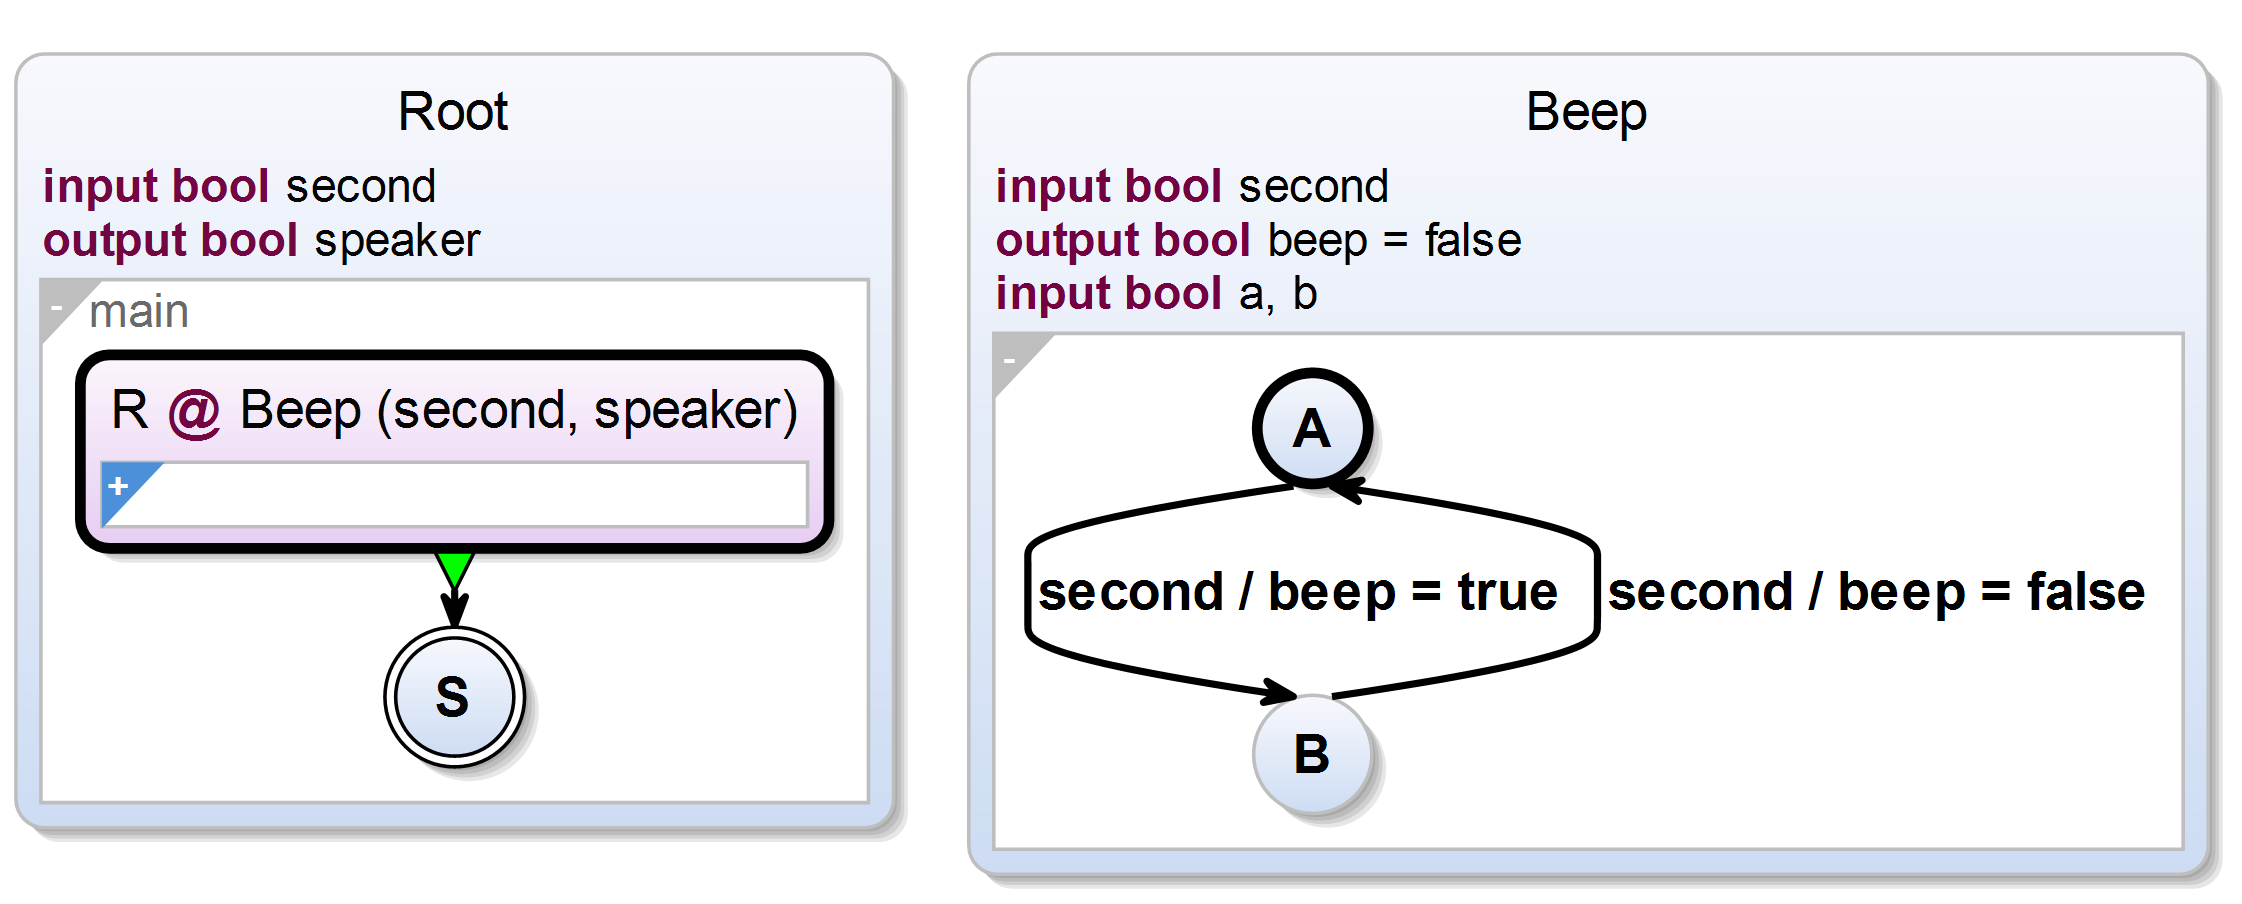
\includegraphics[width=1.0\textwidth]{bilder/BEEP_Reference_Example.png}
\caption{Beep Example for references in SCCharts (adapted from~\cite{.04.09.2023})}
\label{fig:Beep-Reference}
\end{figure} 


\chapter{Related Work}\label{Related_Work}
In this section of the bachelor thesis, related works are addressed. Firstly, reference will be made to similar projects where instances were created using the \textsc{Cinco} Meta Modeling Tool. This is followed by scholarly works that provide more information on MDSD and SCCharts.
\section{Modeling with \textsc{Cinco} related}
For a better understanding of the background of \textsc{Cinco} and the reasons for its development, paper~\cite{Naujokat.2018} provides a comprehensive overview. In addition to the topics mentioned earlier, it also suggests application areas and compares the tool with other meta-modeling tools. Furthermore, it offers a guide on how to create DSLs with \textsc{Cinco}.

In "A Tutorial Introduction to Graphical Modeling and Metamodeling with \textsc{Cinco}" by Lybecait et al.~\cite{Lybecait.2018} presented a \textsc{Cinco} Project that can be used to create web stories, an adventure game. The primary goal was to showcase the two recent additions, Pyro and GCS (Graphical \textsc{Cinco} Specification): Pyro extends the \textsc{Cinco} ecosystem by enabling web-based modeling for \textsc{Cinco}-based graphical modeling languages, while GCS introduces graphical editors to the meta-level in a bootstrapping fashion. This is aimed at reducing the complexity of creating DSLs via \textsc{Cinco} and improving the overall process. The Project can be found here under examples~\cite{.06.05.2022}. 

The second project is a graphical language for statecharts, similar to the one designed in this bachelor thesis. However, instead of using a code generator, an additional simulator for the input was implemented. A screenshot of it can be seen in Figure \ref{fig:CINCO_Statechart_Example} While there is no written thesis available, this project is well-suited for exploring the features of \textsc{Cinco}. It can also be found at~\cite{.06.05.2022} under examples.
\begin{figure}[h!]
\centering
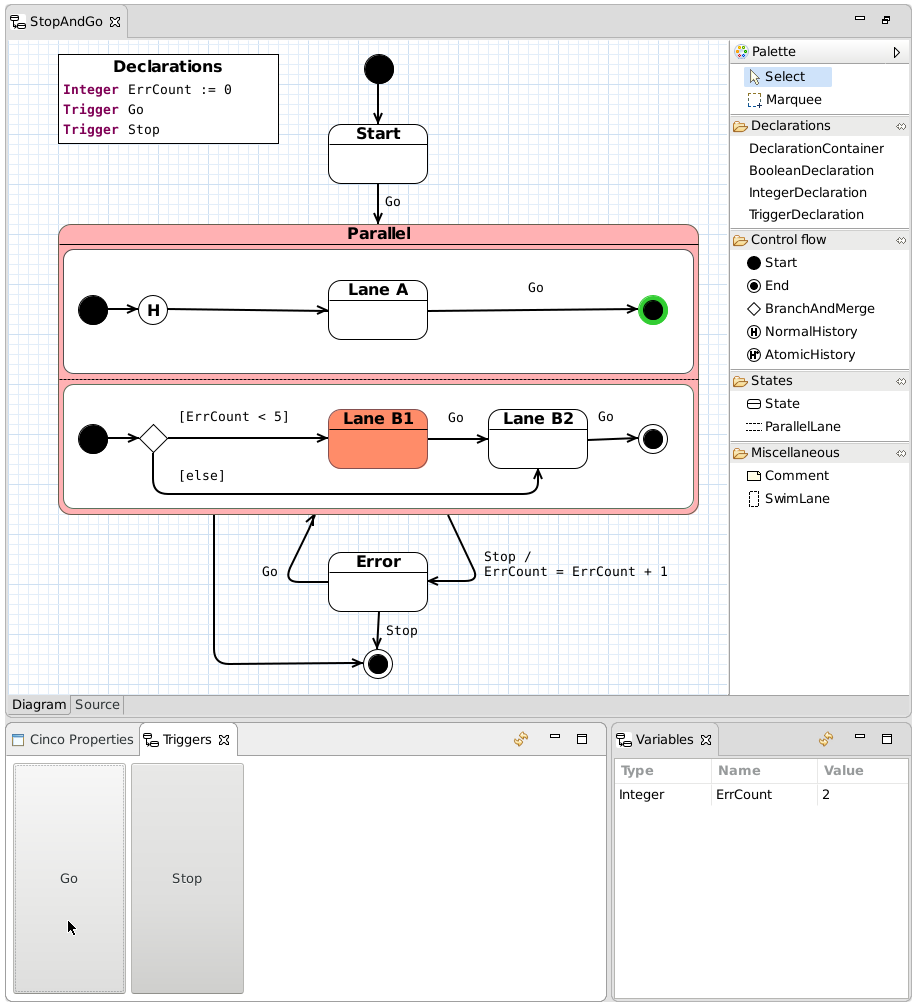
\includegraphics[width=0.8\textwidth]{bilder/CINCO_Statechart_Example}
\caption{StateChart Model and Simulation Screenshot of the \textsc{Cinco} Statechart Project~\cite{.06.05.2022}.}
\label{fig:CINCO_Statechart_Example}
\end{figure} 
\section{Model-Driven-Software Engineering related}
For a very detailed introduction to the topic of Model-Driven Software Engineering, the book by Brambilla, Cabot and Wimmer "MODEL-DRIVEN SOFTWARE ENGINEERING IN PRACTICE"~\cite{Brambilla.2017}, which is often used as a reference here, is highly recommended. In the first section, the authors delve into the basics of MDSE, its use cases, and how to integrate MDSE into existing development processes. In the second section, they delve further into the technical aspects, such as creating a domain-specific modeling language and designing functions for model-to-model and model-to-text transformations.
\section{Sequentially Constructive Statecharts related}
SCCharts have been briefly discussed here to provide a broad overview of this visual language. Some aspects have only been touched upon lightly or not covered extensively to avoid exceeding the scope of this work. For a comprehensive explanation of the SCCharts language and its suitability for implementing safety-critical systems, please refer to Motika's dissertation titled "SCCharts - Language and Interactive Incremental Compilation"~\cite{Motika.2017}. In this source, also detailed explanations of additional features can be found, such as the integration of host code or the pre() operator.
\chapter{Frameworks and Tools}\label{Frameworks_and_Tools}
In this chapter, the most important tools and frameworks used within the context of this bachelor thesis will be introduced. First, Eclipse and Eclipse frameworks related to \textsc{Cinco} are listed, followed by a closer look at \textsc{Cinco}. Finally, a tool for creating SCCharts is introduced.
\section{Eclipse and Frameworks} 
Eclipse is an open-source software project released by IBM since 2001, primarily known as an IDE. However, Eclipse also offers a variety of frameworks and plug-ins that can be easily integrated, thanks to Equinox, an implementation of the OSGi R4 specification.~\cite{Guindon.03.09.2023b} Through the easy integration of these already existing or self-created plug-ins and frameworks, developers can create applications without having to implement complex functionalities themselves.

One of this frameworks is the EMF. It is the central technology within Eclipse for MDSD, as it allows for the design of metamodels using the metamodeling language Ecore. The components of these metamodels can be generated as Java-based code and subsequently customized. Additionally, models can be designed and adapted in a tree-like editor. Furthermore, EMF provides a powerful Application Programming Interface (API). As a result, many other projects in the context of MDSD build upon EMF and offer additional functionalities, such as \textsc{Cinco}.~\cite{Guindon.03.09.2023b}~\cite{Brambilla.2017}

Another framework is Xtext which can be used for the development of programming languages and DSLs, by letting programmers define their own languages via a powerful grammar language. It also offers a well-developed infrastructure which includes linker, parser, typechecker, etc., as well as eclipse integration. 

Xtend is an expressive and flexible java dialect. It compiles in java and thus enables any integration of java libraries. It also offers the function of extending existing types without modifying them, hence the name. It also has the same runtime as equivalent Java code and offers other features such as lambda expressions or template expressions.

\section{\textsc{Cinco} SCCE Meta Tooling Framework}
\textsc{Cinco} is a DSL tool to create domain specific graphical modeling tools. It leverages the extensive metamodeling and infrastructure features provided by the EMF, and the Graphiti diagram editor framework, a modeling infrastructure centered around the EMF, in case for representation and editing.~\cite{Wenz.08.09.2023}~\cite{Naujokat.2018}

Every graphical tool created with \textsc{Cinco}, also called \textsc{Cinco} Product, has at its core the Meta Graph Language (MGL) model, from which the Ecore metamodel is ultimately generated. The MGL also defines which components exists in the model and can be created in the editor at the end. The components are all of the type \textit{node}, \textit{container} or \textit{edge}. Containers are special nodes, which in turn can contain nodes or containers. Both MGL model and the three component types can have attributes, that are structurally similar to declarations in conventional programming languages, with names and data types. In addition, each component of the type node, container and edge has a style. This is defined in the Style Graph Language (SGL). There are \textit{nodestyle} for nodes and containers, and \textit{edgestyle} for edges. A node style is composed of \textit{ContainerShape} and \textit{Shape}. Container shapes can be \textit{roundedRectangle}, \textit{ellipse}, and other geometric shapes. These can contain further container shapes or shapes, such as \textit{text}, \textit{line}, etc. In the edge style, decorations can be defined that are displayed on the connecting line. These can be predefined arrows or circles, but also self-defined decorators. In addition, the \textit{appearance} of each style object, i.e. container shape, shape, edge style or decorator, can be adjusted. This includes, for example, the colour or the line type (solid, dashed, etc.). With the \textit{appearance provider}, the appearance of node styles and edge styles can be changed at runtime. However, with the exception of the appearance, the style can no longer be changed at runtime. This design decision is due to the simplicity approach. 

Besides the MGL and SGL, there are also plug-ins, so-called \textit{meta plug-ins}. These extend the functionality of the editor. They are activated by annotation in the MGL but also in the SGL. An example of such a meta plug-in is the Event API, which enables the editor to respond to various events that occur within it. These events can encompass actions such as node creation, deletion, or resizing. Additionally, events can be triggered when the model is saved or when an attribute is modified. The Event API essentially allows the editor to be more interactive and responsive to user actions and changes in the model. The developer has to imply what should happen after an event. There is also the Prime References meta plug-in, which allows referencing to external components of other models, or the \textit{code generator}, which can be used to generate code from the models. These are just a few of the meta plug-ins from \textsc{Cinco}.

The user interface is shown in Fig. \ref{fig:CINCO_Statechart_Example}. The model created can be seen in the middle. On the right side are the model components nodes and containers, which can be inserted into the model by dragging and dropping. By hovering over nodes or containers, edges can be dragged and dropped into the target node. In addition, the size of nodes and containers can be changed after they have been created. The \textsc{Cinco} properties, in which the attributes of components can be changed, is located in the lower area.

\section{KIELER SCCharts Tool Suite and Compiler Command-Line Interface}\label{Kieler}
The KIELER SCCharts tool suite was developed as part of the Kiel Integrated Environment for Layout Eclipse Rich Client project (KIELER). Using interactive incremental compilation, it provides the user with a better understanding of the compilation process and language features. The user gains more control over compilation in terms of compilation strategy and intermediate results. The modeling language is the SCCharts language.~\cite{Motika.2017}

Fig.~\ref{fig:KIELER_Tool_Screenshot} shows a screenshot of the KIELER SCCharts tool suite. The left window displays the textual editor, where the user can utilize SCCharts Textual Language (SCT) to define corresponding SCCharts. The tool responds to changes in SCT and showcases the generated SCChart in the middle window. The lower window presents the compilation process, offering the user the option to scrutinize individual compilation steps more closely. By clicking on one of the transformations, the interim result is displayed in the middle window. In this case, it represents a transformation from the original (on the left) to Core SCCharts (on the right). However, it's also possible to view the ultimately generated code (e.g., C, Java, etc.) here, depending on the selected target language. Additionally, in the right window, users can customize the layout, enabling configuration of the graphical views of the SCChart.~\cite{Motika.2017}

The KIELER Compiler Command-Line Interface (KIELER Compiler CLI) provides the same functionality as the KIELER SCCharts tool suite but without a graphical user interface. The compiler is accessible from the command line and it takes files in SCT format (*.sctx) as input. Additional parameters can be used to specify the target language, output folder and other settings. Source files and additional information can be found on the project website~\cite{.11.09.2023}.
\begin{figure}[h!]
\centering
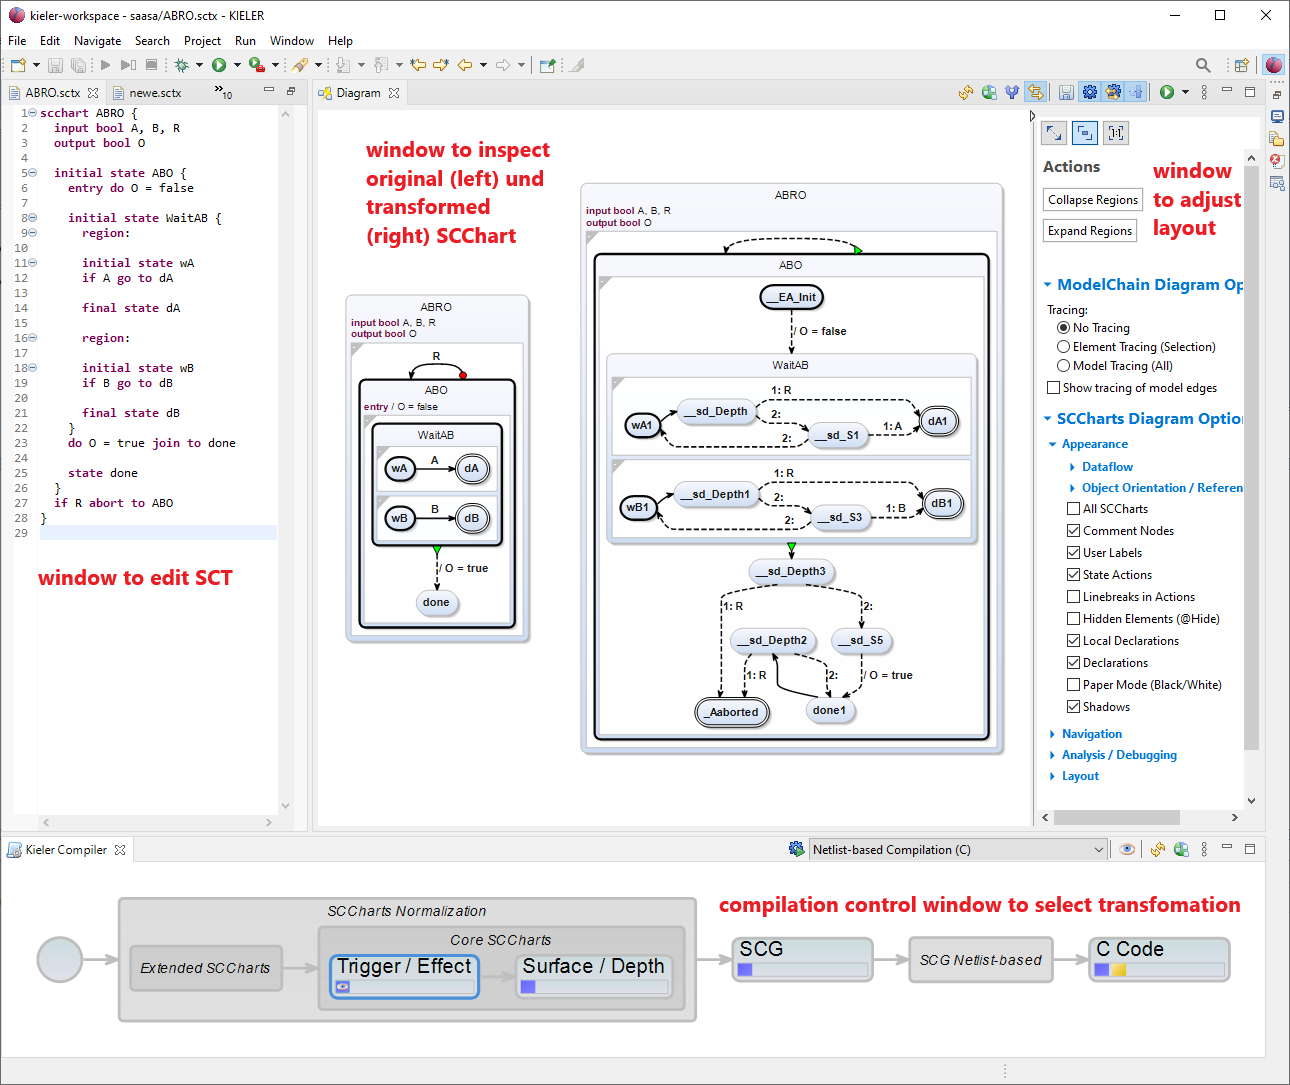
\includegraphics[width=1.0\textwidth]{bilder/KIELER_Tool_Screenshot.png}
\caption{Screenshot of KIELER SCCharts tool (adapted from~\cite{Motika.2017})}
\label{fig:KIELER_Tool_Screenshot}
\end{figure} 
\chapter{Development of the Graph Language} \label{Concept_and_Implementation_of_the_Graph_Language}
In this chapter the concept and implementation of the graphical DSL tool is presented. First, the requirements for the editor are defined, and a suitable data structure with associations and attributes is designed, based on the foundations in Sect. \ref{Sequentially_Constructive_Statecharts}. Subsequently, the MGL is implemented, which uses the designed data structure as a basis. In addition, a style is created in the SGL for each component in the MGL, which defines the appearance of the element in the editor. After that, plug-ins for a better user interface are implemented. Finally, the realization of the code generator is presented, which can generate Java or C code from the created SCCharts models.

\section{Requirements}\label{Requirements}
Before the actual design process of the DSL tool can begin, it is essential to specify the main task and individual requirements, which are elaborated in more detail based on the problem statement.

The following main task results from the problem statement: The development of a graphical DSL tool for creating models of the visual modeling language SCCharts.
To further refine this task, requirements are established. These requirements are derived from considerations of the desired features of the editor. 

The developed tool or editor should be usable for creating models in the SCCharts language. The user interface should be as intuitive as possible, enabling domain experts without programming experience to create models. This means that it should be clear how to create a model, how to adjust and expand existing models, etc.. The editor should provide a palette of modeling elements that align with the specific requirements of the DSL. Therefore, a suitable data structure needs to be identified which can accurately represent the elements of the SCCharts language that are to be modulated. This includes properties or attributes that the components of the SCCharts language possess. Furthermore, the modeling elements should closely adhere to the visual syntax of SCCharts, making it clear which component in the SCCharts language the created element in the editor represents. Additionally, the editor should offer validation functions to ensure that the created models conform to the syntax of the DSL. Errors or inconsistencies should be reported to the user within the editor. A final central feature is that the user should have the ability to generate code in a target language such as Java or C from the created model, which can be utilized to be integrated in software projects. This requires a clear mapping of modeling elements to code constructs.
This results in five core requirements in addition to central ones:
\begin{enumerate}
\item The user interface is intuitive and easy to understand.
\item The underlying data structure correctly represents important relationships and attributes.
\item The visual syntax allow clear identification of the individual components of the SCCharts language.
\item Errors in models are indicated by validation with in the editor.
\item The editor provides code generation from designed models to integrable Java or C code.
\end{enumerate}
Based on these core requirements, designs are now being created to facilitate subsequent implementation.

\section{Data Structure}\label{Data Structure}
A decisive factor in the model transformation is the data structure. This must contain all relevant attributes and associations to adequately represent the elements of the SCCharts language. The correct design of this data structure is of fundamental importance, as it forms the basis for the entire modeling and transformation. First, the individual elements of SCCharts to be implemented within the framework of the editor are examined in more detail, then the relationship between them is examined.

\subsection{Model Elements}
Fig. \ref{fig:Component_Classes} shows all elements of the data structure as classes and subclasses that shall be implemented in the MGL. 
\begin{figure}[h!]
\centering
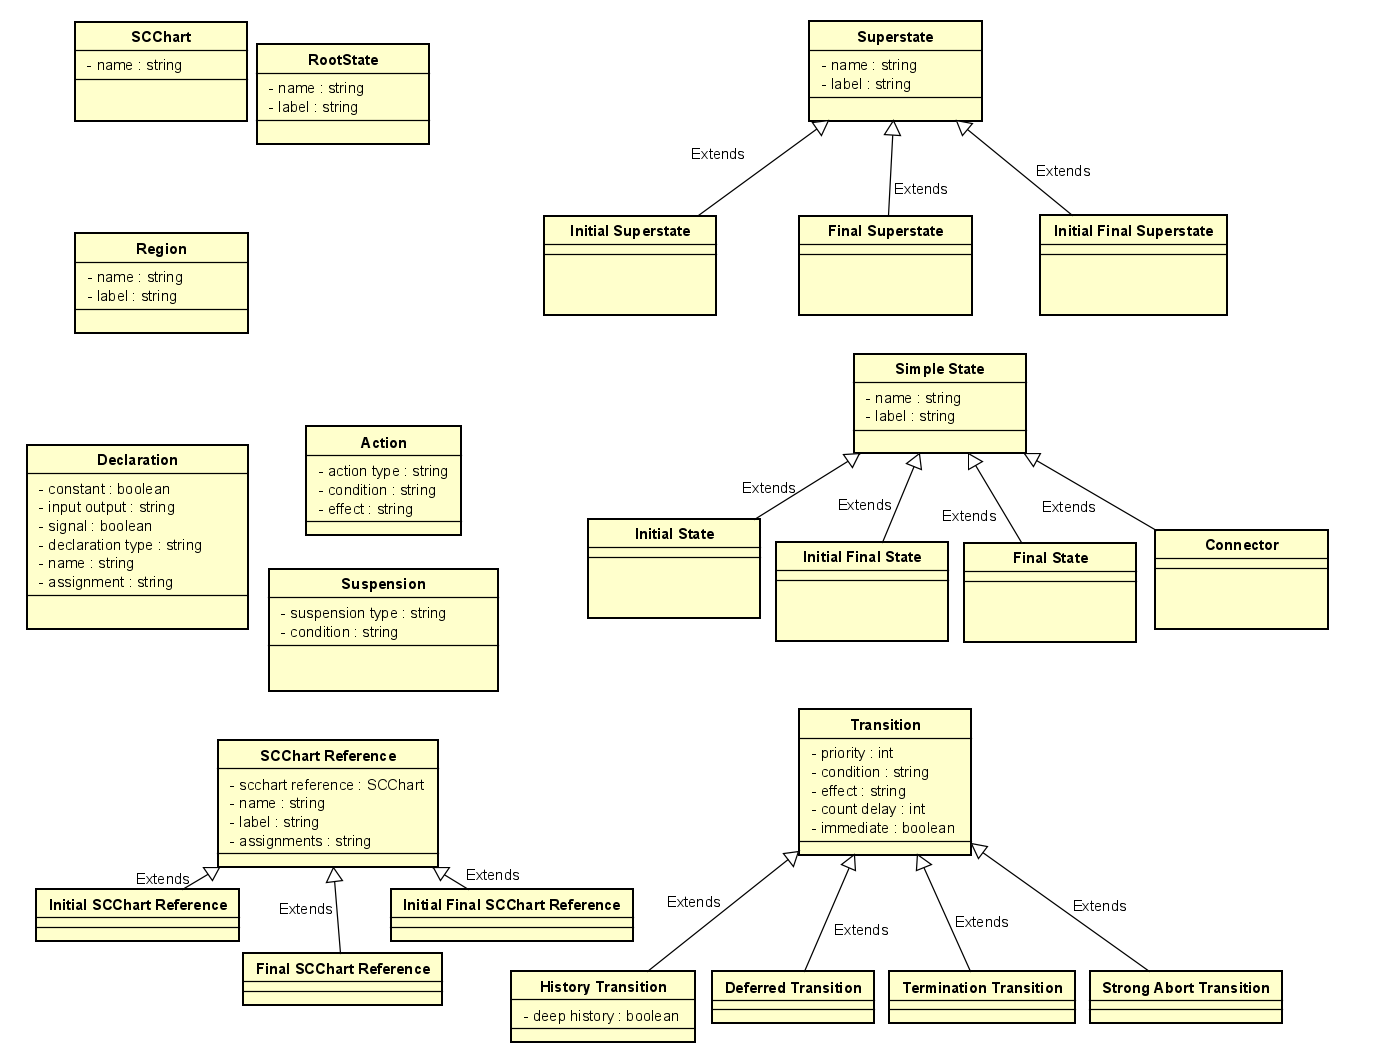
\includegraphics[width=1.0\textwidth]{bilder/Component_Classes.png}
\caption{Classes of the individual components}
\label{fig:Component_Classes}
\end{figure} 
\subsubsection{SCChart, Root State and Region}
The basis is the SCChart model itself, which must have a unique name in form of a string and no other attributes. In addition, there is the root state, of which exactly one exists and which must also have a unique name. Optionally, a label can be added that is displayed as a name when it is set. The same applies to regions, with the exception that here both the name and the label are optional. 
\subsubsection{Superstate and Simple State}
Superstates and simple states are additionally extended by initial, final and initial final states. In the case of simple states, additional connectors are added in the form of a subclass. Each of these states has an individual name and optionally a label, similar to the previously described root state classes.
\subsubsection{Declaration, Action and Suspension}
Declarations can occur on the one hand as constants or signals, which is represented by a boolean value. In addition, they can be declared as input, output, input output or local variable (i.e. none of them). This is made possible by the string data type, as there are more than two options. In addition, they have a name, a declaration type (for datatype) and optionally an assignment, all three of which are represented as strings. Actions and suspensions each have a type and a condition (also known as a trigger), which are defined as strings. In addition, actions have an effect, which is also a string.
\subsubsection{Transition}
Transitions have a priority and a count delay, both of which are represented as integers. In addition, they have a condition (trigger) and an effect (action), which are represented as strings. Furthermore, it is specified whether they are immediate or delayed, whereby this is represented with a boolean value.

The transition class is extended by four subclasses: history transition, deferred transition, termination transition and strong abort transition. The history transition also has a boolean attribute that is used to display deep or shallow history.

In addition to the transition subclasses mentioned, there are other combinations of transition types that are made up of the transition subclasses. An example would be a history transition that is also deferred, i.e. a deferred history transition. This results in a total of twelve different possible transitions. Namely: \textit{transition}, \textit{termination transition}, \textit{strong abort transition}, \textit{deferred transition}, \textit{history transition}, \textit{deferred termination transition}, \textit{deferred strong abort transition}, \textit{termination history transition}, \textit{strong abort history transition}, \textit{deferred history transition}, \textit{deferred strong abort history transition} and \textit{deferred termination history transition}.
\subsubsection{SCChart Reference}
The last component of the data structure is the SCChart reference class. Similar to the superstate class, it has subclasses including initial, final, initial final SCChart references, along with same attributes of the superstate class. Furthermore, it contains a SCChart reference with a SCChart type, and assignments in the form of strings that are necessary for the inputs and outputs of the referenced SCChart.

\subsection{Model Elements Associations and Relations}
Now that the individual components of the data structure have been defined, the relationships and associations between them can be considered. Fig. \ref{fig:ClassDiagramAssociation} represents the class diagram of the data structure that is to serve as the basis for the SCCharts model editor. All associations between the components are illustrated. The fundamental element for this diagram is the SCChart class, which serves as the root element for all other elements. 

The SCChart class contains exactly one root state, which, in turn, contains at least one region and can have an arbitrary number of declarations, suspensions, and actions. Within regions, there can be an arbitrary number of simple states or their subclasses, from which any number of transitions can originate and enter. Furthermore, regions can contain multiple superstates, each of which can have an arbitrary number of regions, declarations, suspensions, and actions. Additionally, an arbitrary number of transitions can connect these elements with others. Lastly, regions can contain any amount of SCChart references, which can, in turn, be linked with an arbitrary number of transitions. Additionally, these SCChart references reference one SCChart.

The created data structure can now be used for the model transformation.
\begin{figure}[h!]
\centering
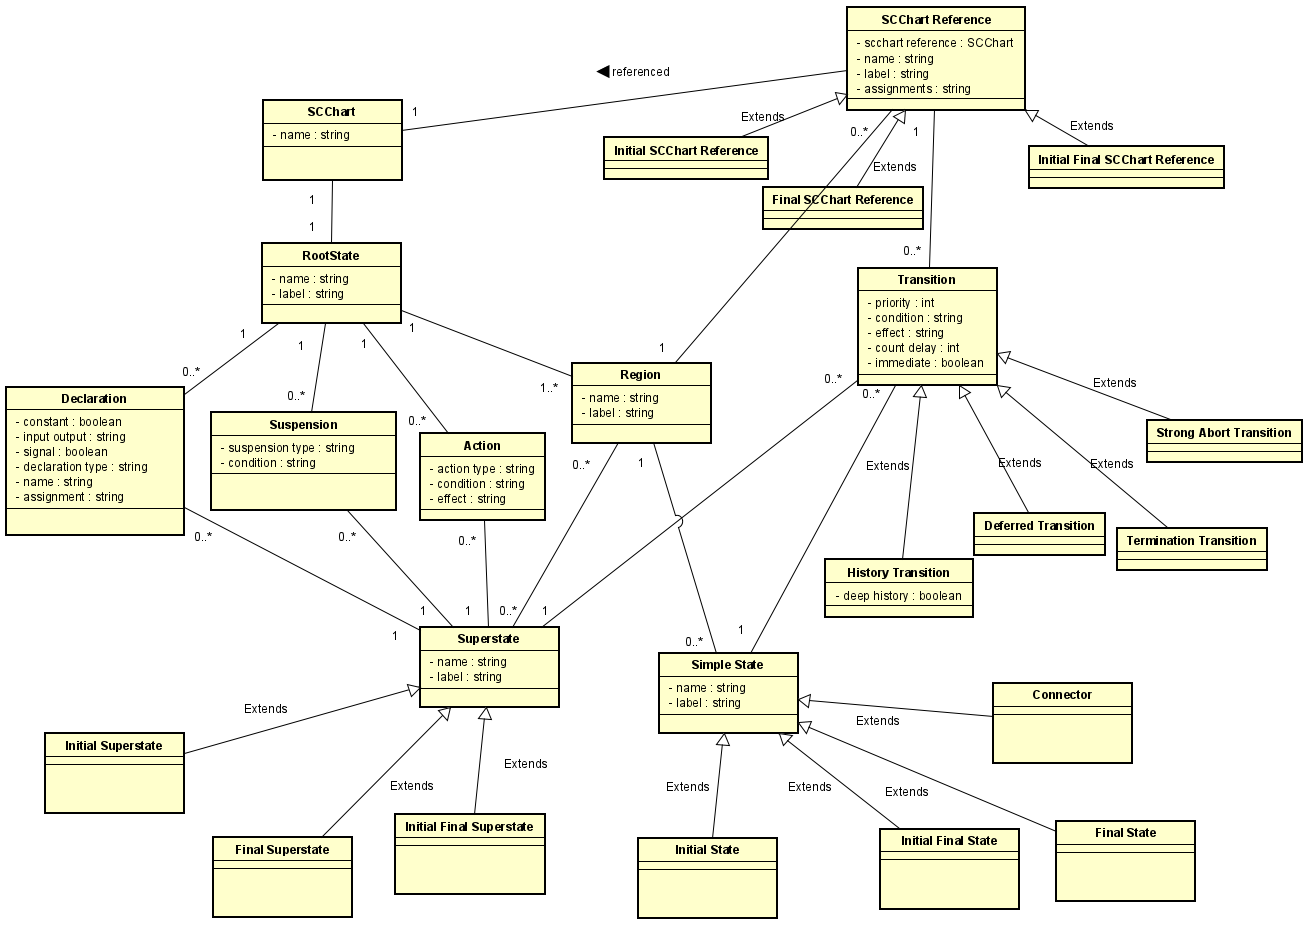
\includegraphics[width=1.0\textwidth]{bilder/ClassDiagramAssociation.png}
\caption{The class diagram of the designed data structure}
\label{fig:ClassDiagramAssociation}
\end{figure} 
\section{Model Transformation}
The model transformation of each \textsc{Cinco} Product is based on the MGL and the MSL, in which all components and their visual representation are defined. In addition to the graph model, the MGL consists of further components of the type node, edge, container. The elements of the designed data structure have to be mapped to the types of the meta graph model of \textsc{Cinco} for the implementation of the MGL. It is crucial to determine which component of the data structure can best be represented by which type of the \textsc{Cinco} meta graph model. 

In Fig. \ref{fig:MappingModelTransformation}, the meta graph model types of \textsc{Cinco} were mapped to the designed SCChart data structure. The class diagram of \textsc{Cinco}'s meta graph model elements can be seen at the top left, with the components graph model (blue), container (green), node (red) and edge (yellow). Below this is the designed SCChart data structure, whose classes have been colour-coded according to \textsc{Cinco}'s meta graph model elements. The graph model was assigned to the SCChart class. All components with inner behaviour, i.e. those that can contain further containers and nodes, are elements of the type container. These include root state, region, superstate and SCChart references. Declaration, suspension, action and simple states, on the other hand, are components of the node type. Transitions were assigned accordingly as edges.

\begin{figure}[h!]
\centering
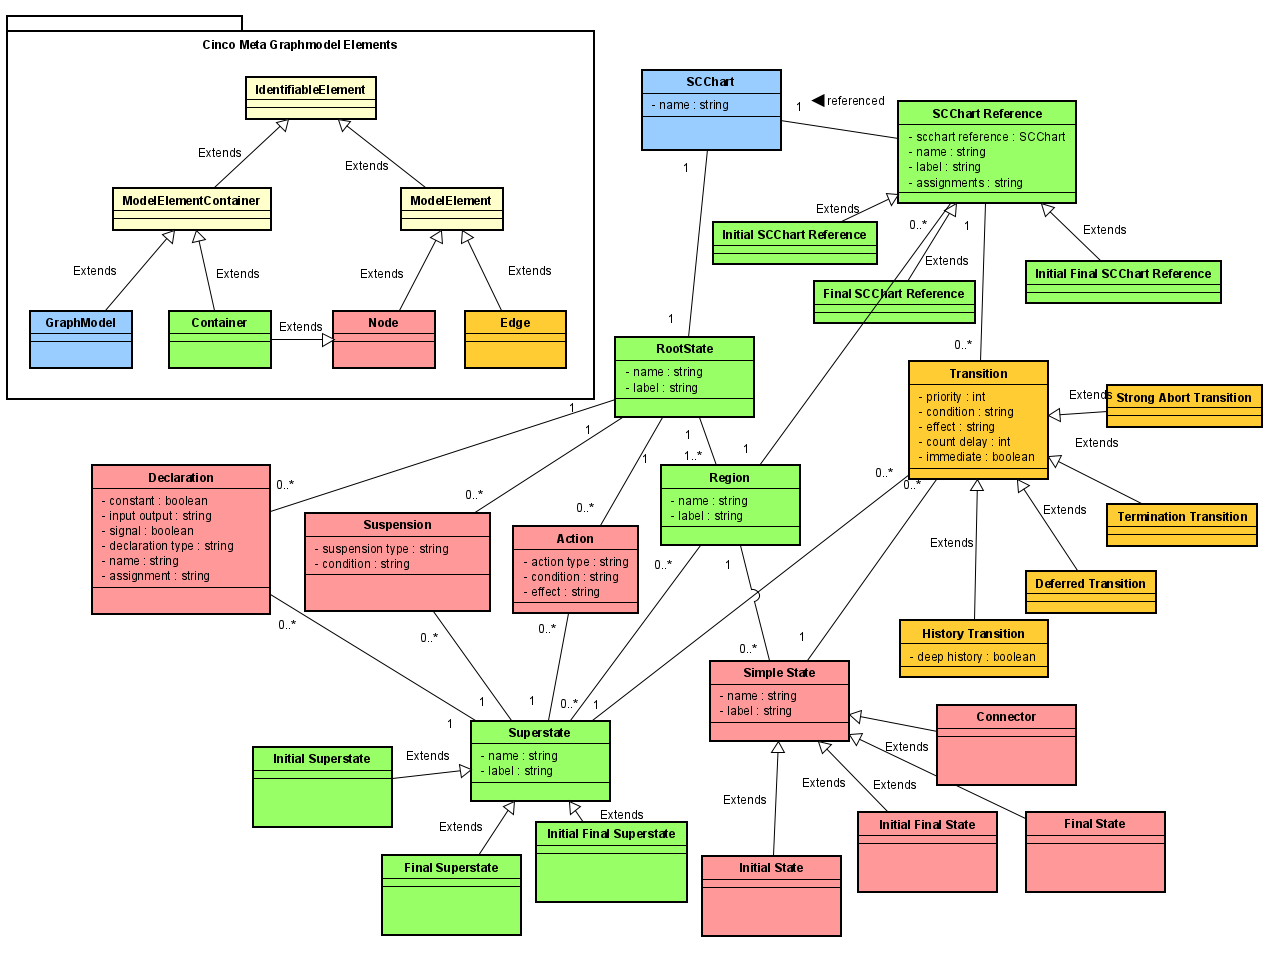
\includegraphics[width=1.0\textwidth]{bilder/MappingModelTransformation.png}
\caption{Mapping of \textsc{Cinco}'s meta graph model elements to the designed data structure for the SCCharts editor}
\label{fig:MappingModelTransformation}
\end{figure} 

\subsection{Implementation of the Meta Graph Language}
With the mapping as a basis, the realisation of the MGL can now begin. All components of the data structure are now implemented with the corresponding \textsc{Cinco}'s meta graph model type. In this section, only one representative for each meta graph model type is considered in more detail, as the implementation for the same types is similar. For the entire implementation of the SCChart MGL, see Appendix \ref{SCChart_MGL}.

\subsubsection{Graph Model}
In Listing \ref{graphmodel_MGL} is the implemented graph model of which there is only one in each MGL. After the keyword \textit{graphModel} the name of the component is given. In this case it is \textit{SCChart}. Then \textit{diagramExtension} is set in each graph model. This determines which file format the created graph model has. Here it is \textit{*.scchart}. \textit{ContainableElements} specifies which components SCChart graph model can contain. The data structure indicates that SCChart model has only one root state. Limits for the number of components can be realised in the MGL using square brackets. In addition, attributes can be defined in graph model, which is done here with name.
\lstinputlisting[frame=single,label=graphmodel_MGL,caption=The SCChart graph model implementation from the SCChart MGL,firstnumber=20,firstline=20, lastline=24]{Code/SCChart.mgl}

\subsubsection{Container}
Superstate was selected here as a representative for a component of the type container. The implementation can be seen in Listing \ref{SuperState_MGL}. All components except the graph model have a style, which is shown here with \textit{style} followed by the name of the style defined in the SGL. The string is an Xtext expression that ensures that if the label of Superstate is set, the label is passed along, otherwise the name. This allows the label for the component to be displayed in the editor if it is specified. Subsequently, in container, as with graph model, \textit{containableElements} can be used to determine which components superstate can contain. According to the data structure for superstate these are regions, declarations, actions, suspensions. \textit{IncomingEdges} and \textit{outgoingEdges} define which transitions can enter and exit. If these are not specified, no transitions can enter or exit. For Superstate, these are all transitions. This could actually be realised with '*', for all edges. However, since an abstract transition is defined in the MGL for the implementation and this should not be included in the model, all transitions must be entered here individually. Finally, the attributes for name and label are defined. For containers, nodes and edges, a class can be extended as usual in programming using the keyword \textit{extends}. In the MGL, the defined properties of the superclass are inherited. In this way, initial superstate, final superstate and initial final superstate are realised, whereby a style must still be specified here.
\lstinputlisting[frame=single,label=SuperState_MGL,caption=The superstate container implementation from the SCChart MGL,firstnumber=62,firstline=62, lastline=69]{Code/SCChart.mgl}

\subsubsection{Node}
In Listing \ref{graphmodel_MGL} the simple state component is shown as a representation for the type node. Nodes have similar properties to containers, except that they cannot contain elements. After the style is referenced, \textit{incomingEdges} and \textit{outgoingEdges} can be set, which are fewer compared to superstates. Although this is not directly evident from the data structure, it makes sense when considering the functions that some transitions have when entering or exiting a state. Since simple states have no internal behaviour, such transitions have no effect on them and would therefore be rather confusing. For this reason, the deferred and history transitions are missing from the incoming edges, and the strong abort and termination transitions are missing from the outgoing edges. Subsequently, attributes can be specified, in this case the name, which is already initialised, and the label. Initialising name with \textit{<set name>}, which has already been done for superstates, is to ensure later that the user gives the state a unique name.
\lstinputlisting[frame=single,label=SimpleState_MGL,caption=The simple state node implementation from the SCChart MGL,firstnumber=132,firstline=132, lastline=138]{Code/SCChart.mgl}

\subsubsection{Edge}
To better distinguish (normal) transition from other transition types, the superclass abstract transition was added, from which all twelve transition types inherit. Listing \ref{DeferredHistoryTransition_MGL} shows the implementation of the deferred history transition. The string contained in the referenced style is an Xtext expression with the function that the label of the edge has the format '[priority:] [[count delay] condition] [/ effect]'. Only the attributes of the label that have been set are displayed within the label. A second string is given for history transitions that is used for displaying deep history. Besides style, only attributes for edges can be defined.
\lstinputlisting[frame=single,label=DeferredHistoryTransition_MGL,caption=The deferred history transition edge implementation from the SCChart MGL,firstnumber=280,firstline=280, lastline=287]{Code/SCChart.mgl}

\subsubsection{Prime Viewer Meta Plug-In}
Listing \ref{PrimeViewer_MGL} shows the Prime Viewer plug-in. It is used to implement the reference in the data structure from the SCChartReference to an SCChart model. This must be activated before the graph model with the annotation \textit{@primeviewer}. Afterwards the annotation \textit{@pvFileExtension(...)} can be used to search for files of this format which contain the referenced model element. In this case the file extension is \textit{scchart} and the model element is SCChart. This is then assigned to \textit{reference}, which basically behaves like an attribute and contains all the information of the referenced SCChart.
\lstinputlisting[frame=single,label=PrimeViewer_MGL,caption=The Prime Viewer meta plug-in for SCChart reference,firstnumber=166,firstline=166, lastline=178]{Code/SCChart.mgl}

\subsection{Implementation of the Style Graph Language}
The visual appearance of the components from the MGL is defined in the MSL. In node styles, the visual representation of components of the type node or container can be defined and in edge style for components of the type edge. In this section, only one representative each of the node style and the edge style will be examined in more detail, as the implementation process of these styles is highly repetitive. For the entire implementation of the SCChart SGL, see Appendix \ref{SCChart_SGL}. In general, it is tried to stay as close as possible to the original syntax and visual representation of the SCCharts language with the given graphical elements and the settings of the appearance of the SGL.

\subsubsection{NodeStyle}
In node style, any number of container shapes, such as rounded rectangle or ellipse, or shapes such as text or polylines, can be defined. Container shapes can also contain other container shapes and shapes. Listing \ref{initialFinalSuperStateStyle_SGL} shows the node style of the component initial final superstate. The number in the bracket after the name determines the number of string parameters that must be provided by the components of the MGL. The name or label of the initial final superstate from the MGL is passed here. Then a container shape is implemented with \textit{roundedRectangle} and its appearance is determined with \textit{initialFinalStateOuterCircle}. In this case, it is a little wider line to indicate the initial feature. Then the size is set with \textit{size()} and the rounded corners with \textit{corner()}. In addition, another inner rounded rectangle is defined whose appearance determines the fore and background colour. With \textit{position} the location of the inner rectangle can be set in the outer rectangle. The size and the rounded corners can be adjusted as for the outer rectangle. Thus, the component has a double border indicating the final feature. In the inner rectangle, a text is defined that receives the parameter string and displays it in the middle at the top of the inner rectangle. The visual representation in the editor of the initial final superstate is shown in Fig. \ref{fig:SGL_Elements} left.
\lstinputlisting[frame=single,label=initialFinalSuperStateStyle_SGL,caption=The initial final superstate style implementation from the SCChart SGL,firstnumber=163,firstline=163, lastline=180]{Code/SCChart.style}

\subsubsection{EdgeStyle}
In edge styles, the appearance of the connecting line and the decorators can be defined. As with node style, a string must be given as argument for termination transition, as shown in Listing \ref{terminationTransitionStyle_SGL}. The appearance provider is used for every transition type to change the line of the edge from solid to dashed on runtime if the transition is immediate, i.e. the boolean \textit{immediate} is true. In this way, it is not necessary to define an equivalent immediate transition type in the MGL for each transition type. Furthermore, termination transitions are also displayed as dashed transitions if they are unconditional. The referenced class of the Appearance Provider is an Xtend class for each transition type, in which the function when to change the appearance is implemented. After that, the default appearance is set. In addition, decorators are defined that lie on or at the line. These can have predefined shapes like the first decorator (arrow). The location also specifies the relative position of the decorator to the edge. An appearance can also be specified for each decorator. The second decorator is a self-defined green triangle at the beginning of the transition, which indicates the termination of the source state. The last decorator displays the text, i.e. the label of the edge, which includes priority, condition, count delay and effect. This is displayed in the centre and can be moved because of the \textit{movable} keyword. The representation of the termination transition in the editor is shown right in Fig. \ref{fig:SGL_Elements}
\lstinputlisting[frame=single,label=terminationTransitionStyle_SGL,caption=The termination transition style implementation from the SCChart SGL,firstnumber=347,firstline=347, lastline=369]{Code/SCChart.style}

\begin{figure}[h!]
\centering
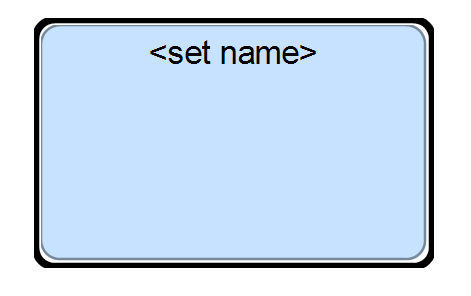
\includegraphics[width=0.5\textwidth]{bilder/SGL_InitFinSuper_Shape.png}
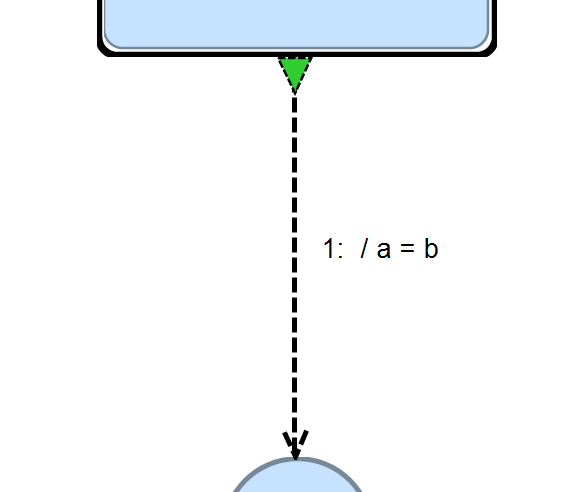
\includegraphics[width=0.4\textwidth]{bilder/SGL_TermTran_Shape.png}
\caption{Visual representation of the initial final superstate (left) and the termination transition (right) in the editor}
\label{fig:SGL_Elements}
\end{figure} 

\section{User Interface and Model Validation}
Although it is already possible to create SCChart models with the implementation of MGL and SGL, the editor, in its current state, would not provide a good user experience. The issue is illustrated in Fig. \ref{fig:Bad_User-Interface}. All components of the type container and node are listed under the \textit{node} tab on the right-hand side. A model with several components has been created in the middle. When components are created by drag and drop, they are created at the location where they are dropped with the specified size defined in the SGL. This may mean that the component created is too large for the container or that the component should not be displayed in this position. This can lead to the creation of confusing diagrams. It is also tedious to have to manually adjust the nodes and containers every time when creating new components or deleting old ones. The KIELER SCChart tool suit (Sec. \ref{Kieler}) has an automatic layout which, when designing SCCharts after changes to the SCT, automatically arranges the model appropriately. Within the scope of this bachelor thesis it is not possible to realise such a comprehensive layout program. But with the meta plug-ins from \textsc{Cinco}, the usability of the editor can be improved with little effort. Therefore, it would be useful if declarations, suspensions and actions were arranged in a superstate or root state directly in the upper area when they are created and the remaining declarations, suspensions and actions are rearranged when they are deleted in order to close any gaps that occur. The same applies to regions. These are to be integrated next to other regions with the same distance to them or also to the border when they are created. In addition, not all functions such as resizing, deleting or moving should be possible for all components, as e.g. simple states should have a constant size. In the next sections, meta plug-ins and their implementation are presented, which improve the user-friendliness of the editor.

\begin{figure}[h!]
\centering
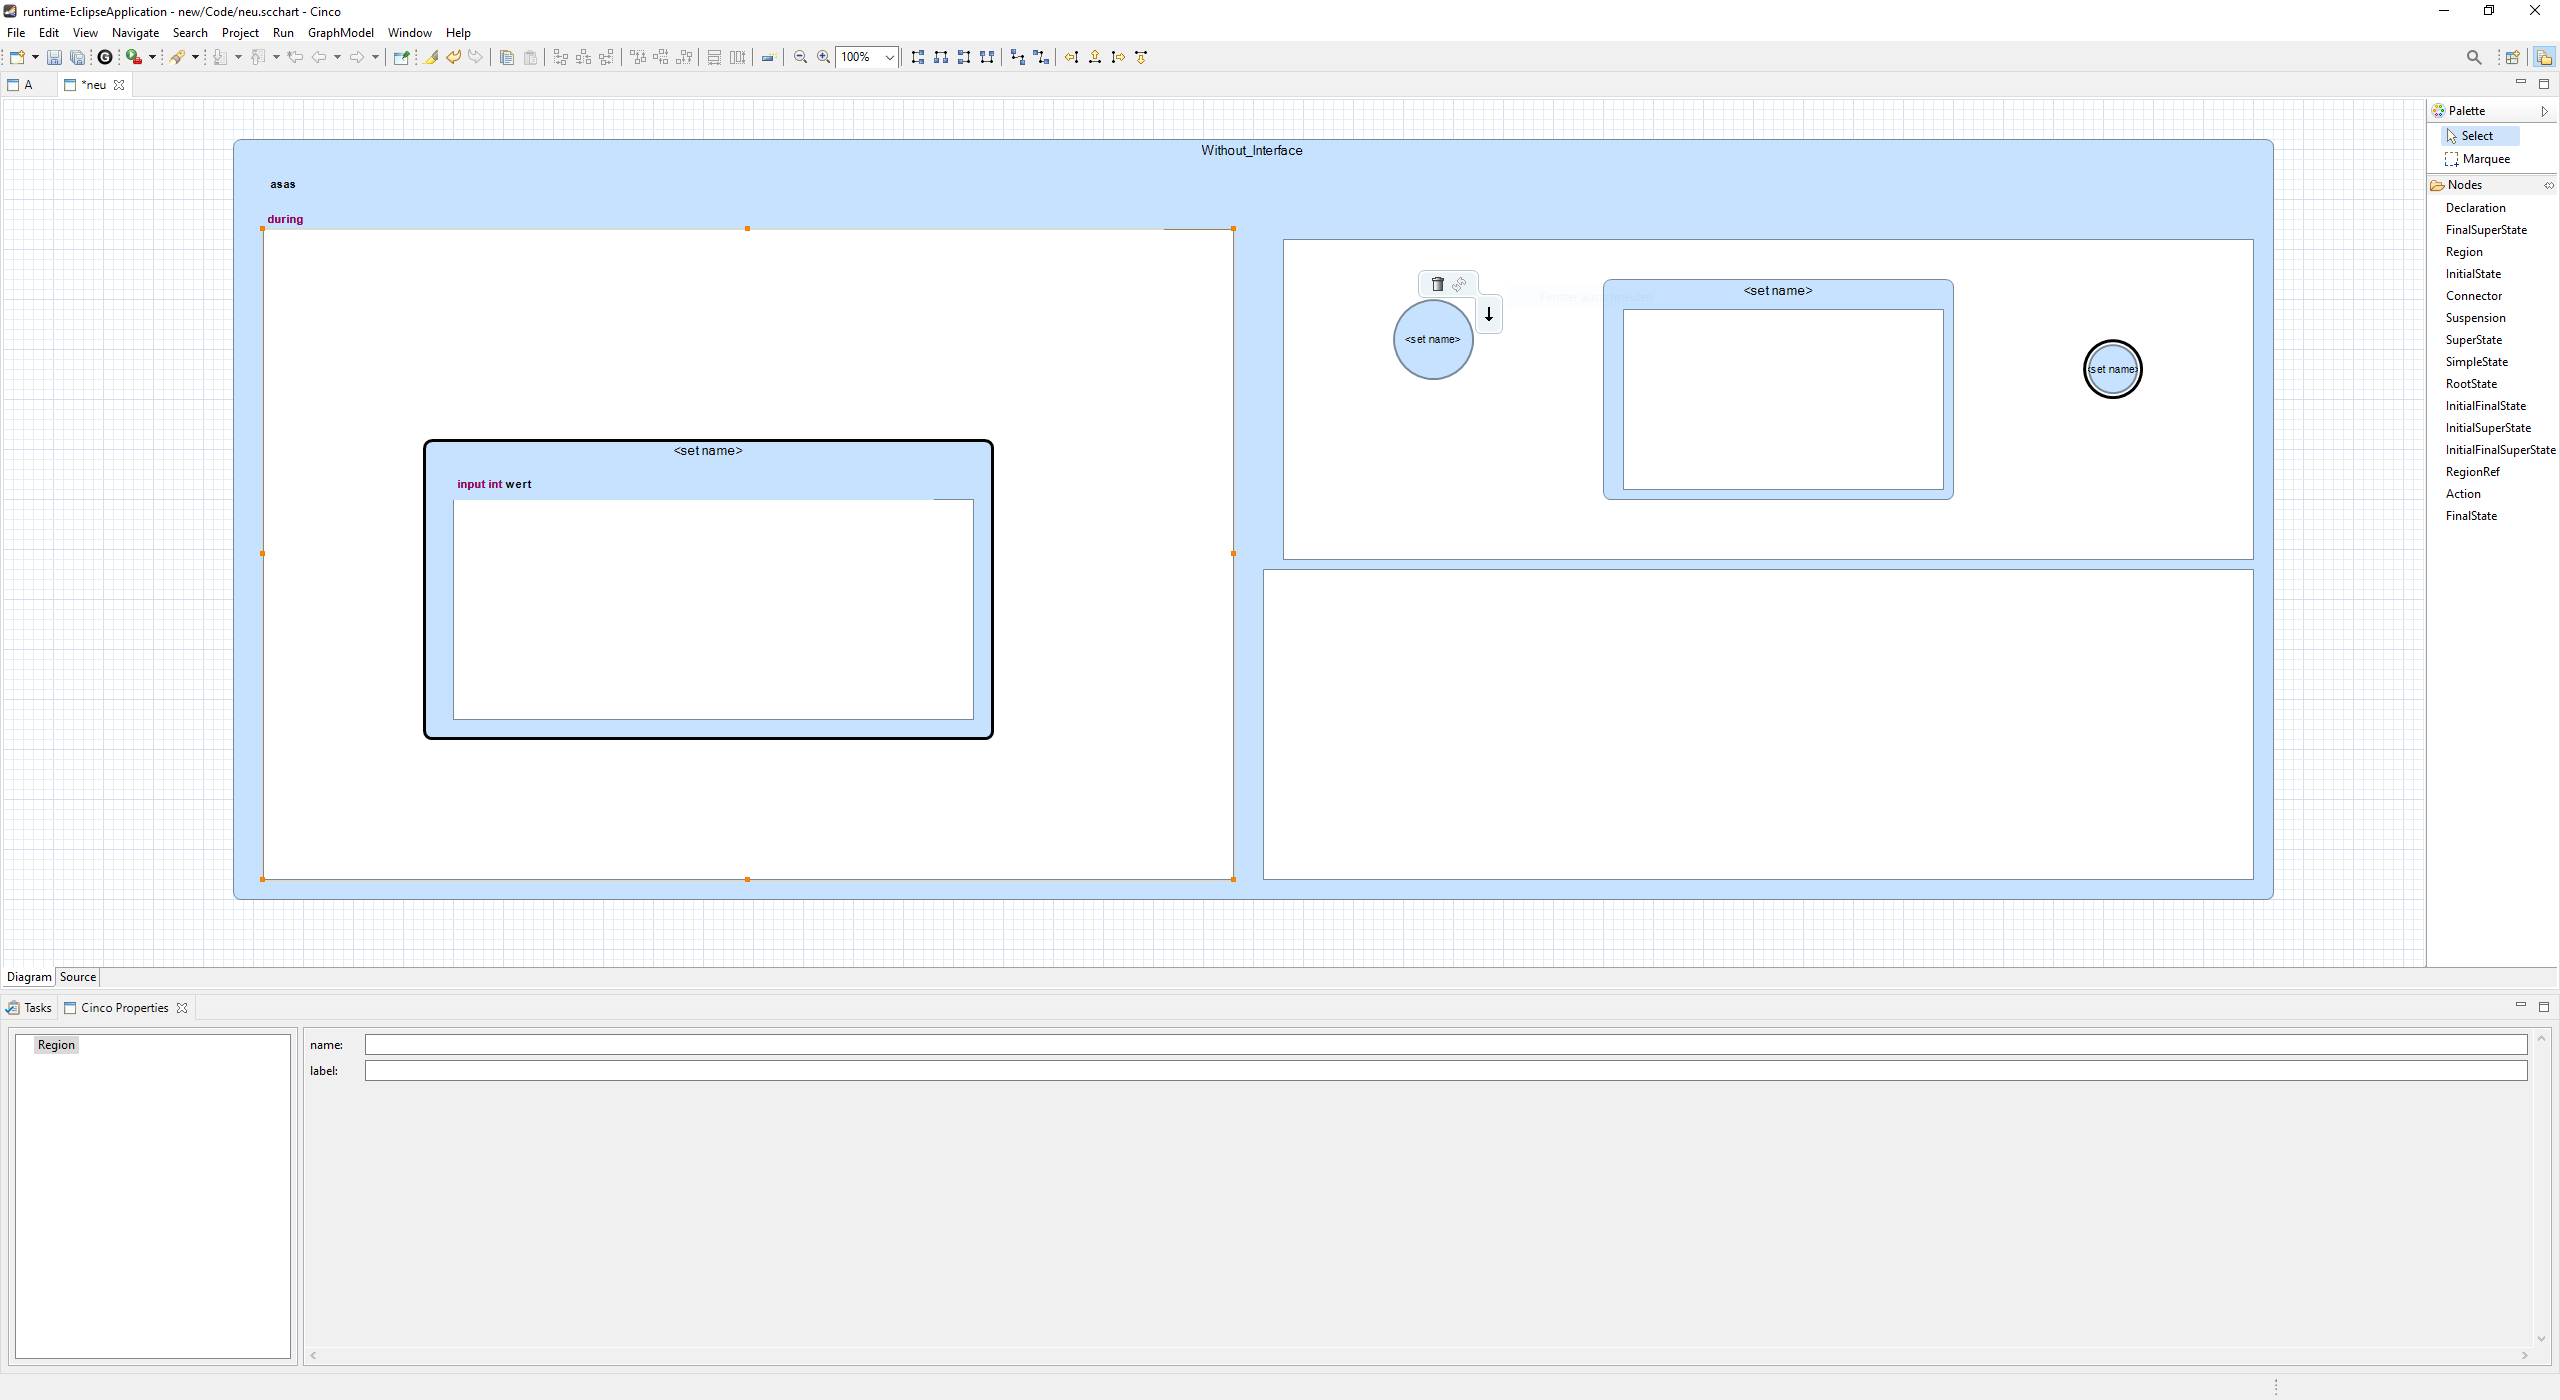
\includegraphics[width=1.0\textwidth]{bilder/Bad_User-Interface.png}
\caption{The SCCharts editor without plug-ins}
\label{fig:Bad_User-Interface}
\end{figure} 

\subsection{Event API}
The Event API can be used to react to various events in the editor. These events can be, for example, the creation or moving of a component. The Event API can be activated for a component in the MGL by annotation and can be applied to all component types. In the corresponding event class of the component, the functionality can be implemented for an event.

For the SCChart graph model, the Event API is used to automatically create a root state with a region after creation. This is because every SCChart has a root state. Furthermore, for superstates and the root state, regions, declarations, suspensions and actions are automatically adjusted to the new size of the superstate or root state after a change in size. 


In order for declarations, suspensions and actions to be listed in the upper left corner of their associated states, within the Event API a function is implemented for each component, which is called when the respective component is created. Listing \ref{actionPostCreate} shows, as an example, a part of the code implemented for the \textit{postCreate} event of action. For the arrangement of the elements in the respective states, these must be accessed. Since the superstate or root state cannot be accessed directly as the respective instance, the SCChart model is called via the method \textit{rootElement} and then the state that contains the created action node is identified via a tree-like search. To identify the state containing the created action node, a random UUID is assigned via the Java UUID (Universally Unique Identifier) class when the action node is created (line 34). This requires an additional attribute to be defined in the MGL for actions. To make it invisible to the user of the editor, it is hidden in the editor with the annotation \textit{@propertiesViewHidden}. The algorithm first iterates the root state and searches in the list of actions (if not null) for an element with the UUID of the created element (lines 36-38). If the action node with the UUID is found in the root state, action nodes are reordered with the created action (lines 39-51). To do this, the number of declarations and suspensions are first determined (lines 39-45) in order to be able to place the action nodes below them. Then a check is made to see if a region has been obscured by the placement of the action node. If this is the case, the region is reduced accordingly (lines 53-60). If the created action is not in the root state, the superstates in the regions of the root state are searched for the element (lines 65-73). The method \textit{postCreateAction()} (line 69) is similar in structure to \textit{postCreate()} (line 33). The only difference is that the action node created is searched in a superstate and instead in a root state. This method is also recursive, i.e. in each superstate in which the element was not found and in whose regions there are still superstates, the function is called again for the superstates contained. Similar methods were used for post creations of declarations or suspensions. And similar procedures are also implemented for post deletion of corresponding components, which ensure that no gaps exist within declarations suspensions and actions, and regions resize accordingly when space is freed up at the top of the state. For the entire implementation of the Xtend ActionEvent class, see Appendix \ref{ActionEvent_Xtend}.
\lstinputlisting[language=xtend,frame=single,label=actionPostCreate,caption=Part of the implementation in Xtend for the postCreate method of the action event class,firstnumber=33,firstline=33,lastline=74]{Code/ActionEvent.xtend}

The Event API is also used to arrange regions when they are created in a state. Again, the root state or superstate in which the region is created must be accessed, so a similar search algorithm is used as for actions. For this, region also receives a hidden UUID attribute in the MGL. If state containing the created region is found, the region next to it (if exists) is halved (minus the distance between them) and the region created is placed on the area that becomes free with the same size as the halved region. For better understanding an example for this is shown in \ref{fig:Event_region}. The arrows indicate on which side the new region was created and what the superstate looks like after the regions have been arranged. If a region is created between two regions, the left or upper region is first used to create the new region. If there is no region in the state, the created region will have the entire size of the state minus the distance to the borders. During the implementation, cases occurred where the region was simply placed but not arranged, which could lead to the creation of incorrect models. For this case, the algorithm was extended so that the region is deleted automatically if it is not arranged, so that the user can try to create a new region again. For the post delete function of regions, the create function is basically reversed. Again, the state that contained the deleted region is searched first, and then a neighbouring region of similar size to the deleted region is searched for. In this way, the region takes up the area of the deleted region without covering other regions or leaving free areas in the state. With these simple methods of the event classes, components can be dynamically created, deleted and resized.
\begin{figure}[h!]
\centering
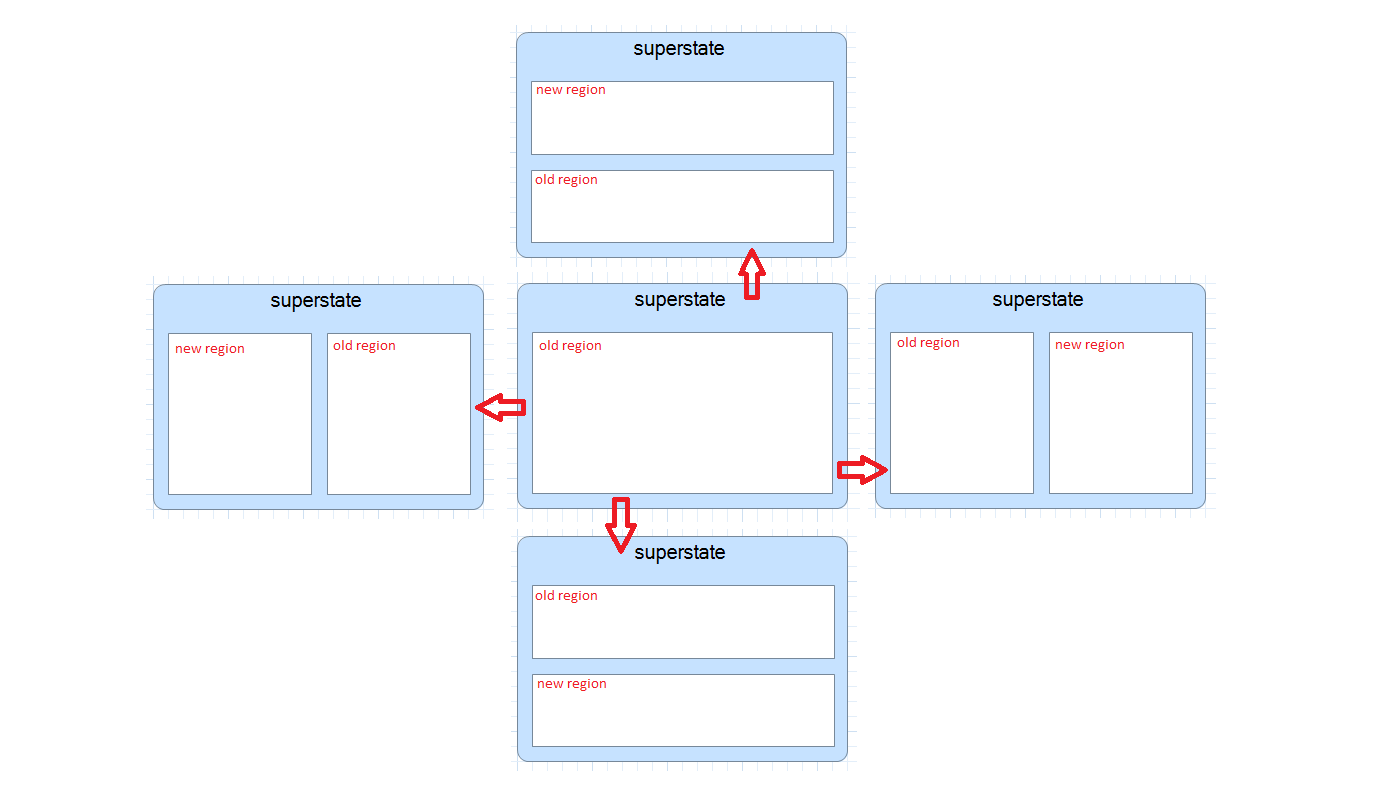
\includegraphics[width=1.0\textwidth]{bilder/Event_region.png}
\caption{Ordering mechanism of created regions in states}
\label{fig:Event_region}
\end{figure} 

\subsection{Palette, Disable, Possible Value Provider}
Besides the Event API, which can be used to implement many different functions, there are also smaller plug-ins that can be applied to improve the user interface. These are briefly presented below.

With the palette plug-in, containers and nodes can be grouped under their own term on the right-hand side of the editor, which improves clarity for the user. For example, superclasses can be combined with subclasses under the\textit{Superstates} tab. In addition, components can be hidden if no term is specified in the palette name. This is used for the root state, as it only exists once in SCChart and is created directly when an SCChart model is created via the Event API.

In the editor it is desirable that certain functions such as resize or move are not available for some components. Otherwise, the user can make changes to the model that are not intended. \textit{@disable} can be used for this purpose by disabling the functions move, select, create, resize and delete in the editor for certain components. Thus, resize is disabled for simple states and their subclasses, as their size should be adjustable. Furthermore, move and resize are disabled for region and declarations, suspensions and actions, as their arrangement and resizing is controlled by the Event API. In addition, delete has been disabled for root state, as the user should not be able to delete it.

The Possible Value Provider plug-in can be used to specify certain values for attributes of components to ensure that users cannot make invalid entries. This is used in declarations, actions and suspensions, e.g. to define the type. In addition, the possible selection of the priority of outgoing transitions for states is defined, whereby the selection option is bound to the number of outgoing edges.

\subsection{Model Compare and Merge Framework}
The Model Compare and Merge (MCaM) framework can be used to perform validations during model creation in the editor. To do this, it is activated with \textit{@mcam("check")} in the MGL. Subsequently, with \textit{@mcam\_checkmodule()} the classes in which the validations are implemented are registered in the MGL. For a better overview during implementation, it makes sense to create a separate check module for each class or superclass of the MGL.

Thus, a priority check for transitions is implemented, which checks whether the outgoing edges of each node and container of the model have a valid priority. A further function checks whether the source and target elements of a transition are in the same region. Another example is the check for regions that must always have exactly one initial state, initial superstate or initial SCChart reference. Other, but certainly not all, checks are implemented.


\section{Implementation of the Code Generator}
After the user interface has been adapted and validation functions realised, models can now be created. To be able to convert these models into C or Java code, a code generator must be implemented.

The Generatable meta plug-in of \textsc{Cinco} is a tool, that utilises template expressions of Xtend and can be used to attempt to translate SCChart models into Java or C code. However, this would be elaborately, as it is not so easy to translate the features of the SCCharts language into corresponding Java and C code artefacts. A simpler method is to use the KIELER Compiler CLI from Sect. \ref{Kieler}, which can generate C or Java code from SCT. This means that the components of the model would have to be converted into SCT format using the code generator and then passed to the KIELER Compiler CLI.
In Fig. \ref{fig:SCChartsCheatSheetMod} Core SCCharts and Extended SCCharts are shown with SCT translations for each component in the margin. Most of the SCT translations are already illustrated here. The only missing component are the SCChart references, which need to be called at the beginning of an SCT file with an import statement, and further defined in a second call. 

\begin{figure}[h!]
\centering
\includegraphics[width=1.0\textwidth]{bilder/SCChartsCheatSheetMod.png}
\caption{Core- and Extended SCCharts with SCT annotation~\cite{.06.05.2022}.}
\label{fig:SCChartsCheatSheetMod}
\end{figure} 

For the model to text transformation, a function is defined for each component in the code generator plug-in, as shown in Fig. \ref{fig:CodeGenClasses}. This function is responsible for placing keywords and attributes of its component at the appropriate location in the SCT file. For components of type container, the containing components are invoked along with their defined functions.

To show what such a function looks like, Listing \ref{CodeGenTemp} shows the template function that is used to translate the root state of the SCChart graph model into SCT. The generation of the other components of the SCChart model originates from here. ''' in line 60 indicates that this is a template expression, i.e. text indentation is taken into account outside the french prefixes.  In lines 61-63, the imports for possible referenced SCCharts are converted. Then follows the formatting for the root state with \textit{scchart} as the keyword and, separately, the name of the root state. Within the curly brackets, the declarations, suspensions, actions, and regions contained in the root state in this order are then called with the corresponding functions (lines 65-84). 
\lstset{literate=
  {á}{{\'a}}1 {é}{{\'e}}1 {í}{{\'i}}1 {ó}{{\'o}}1 {ú}{{\'u}}1
  {Á}{{\'A}}1 {É}{{\'E}}1 {Í}{{\'I}}1 {Ó}{{\'O}}1 {Ú}{{\'U}}1
  {à}{{\`a}}1 {è}{{\`e}}1 {ì}{{\`i}}1 {ò}{{\`o}}1 {ù}{{\`u}}1
  {À}{{\`A}}1 {È}{{\`E}}1 {Ì}{{\`I}}1 {Ò}{{\`O}}1 {Ù}{{\`U}}1
  {ä}{{\"a}}1 {ë}{{\"e}}1 {ï}{{\"i}}1 {ö}{{\"o}}1 {ü}{{\"u}}1
  {Ä}{{\"A}}1 {Ë}{{\"E}}1 {Ï}{{\"I}}1 {Ö}{{\"O}}1 {Ü}{{\"U}}1
  {â}{{\^a}}1 {ê}{{\^e}}1 {î}{{\^i}}1 {ô}{{\^o}}1 {û}{{\^u}}1
  {Â}{{\^A}}1 {Ê}{{\^E}}1 {Î}{{\^I}}1 {Ô}{{\^O}}1 {Û}{{\^U}}1
  {ã}{{\~a}}1 {ẽ}{{\~e}}1 {ĩ}{{\~i}}1 {õ}{{\~o}}1 {ũ}{{\~u}}1
  {Ã}{{\~A}}1 {Ẽ}{{\~E}}1 {Ĩ}{{\~I}}1 {Õ}{{\~O}}1 {Ũ}{{\~U}}1
  {œ}{{\oe}}1 {Œ}{{\OE}}1 {æ}{{\ae}}1 {Æ}{{\AE}}1 {ß}{{\ss}}1
  {ű}{{\H{u}}}1 {Ű}{{\H{U}}}1 {ő}{{\H{o}}}1 {Ő}{{\H{O}}}1
  {ç}{{\c c}}1 {Ç}{{\c C}}1 {ø}{{\o}}1 {Ø}{{\O}}1 {å}{{\r a}}1 {Å}{{\r A}}1
  {€}{{\euro}}1 {£}{{\pounds}}1 {«}{{\guillemotleft}}1
  {»}{{\guillemotright}}1 {ñ}{{\~n}}1 {Ñ}{{\~N}}1 {¿}{{?`}}1 {¡}{{!`}}1 
}
\lstinputlisting[language=xtend,frame=single,label=CodeGenTemp,caption=Template function of the SCChart code generator,firstnumber=60,firstline=60,lastline=86]{Code/CodeGenerator.xtend}

In SCT, priority is regulated so that transitions with the highest priority are placed directly after the source element, followed by transitions with the second-highest priority, and so on. For this purpose, an extra function, \textit{genEdgesOrder(...)}, is implemented that outputs the transitions for components with outgoing edges in the correct order after the component. The generated file with the file extension *.sctx is saved in the folder specified in the MGL in the workspace. 

In addition, a command line call with the method \textit{commandLineParser} is implemented, that invokes the KIELER Compiler CLI and passes the generated file in SCT format along with instructions for the target language as parameters and target directory. The target directory is the folder in which the SCT file is located. The KIELER Compiler CLI offers different compilation variants for Java and C. It also offers the possibility to convert the SCT file into a diagram, which can be useful for validating the created model with the editor. In total, there are seven different types of compilation. For this reason, another attribute is defined in the MGL for root state, which is used in the editor to select the target language of the code generator. The plug-in Possible Value Provider is used for this purpose. With this, the user can select one of the possible compilation types. This code generator is written for the Windows operating system, as it calls the \textit{cmd.exe}. However, it can easily be implemented for other operating systems by calling the appropriate terminal application.

\begin{figure}[h!]
\centering
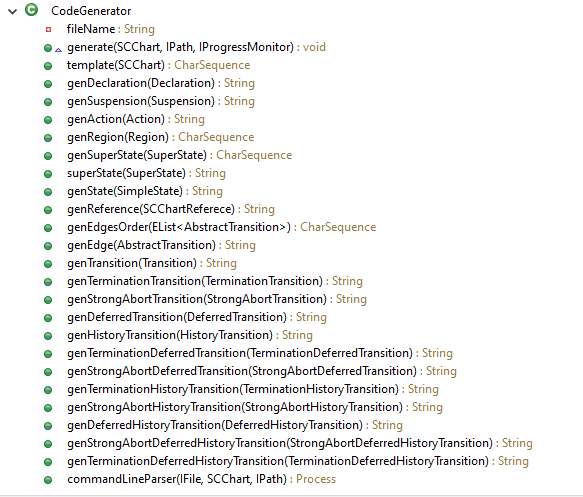
\includegraphics[width=1.0\textwidth]{bilder/CodeGenClasses.png}
\caption{Methods of the implemented Xtend class from code generator plug-in}
\label{fig:CodeGenClasses}
\end{figure} 


\chapter{Evaluation of the Model Editor} \label{Evaluation_of_the_Model_Editor}
In this chapter, the created editor is evaluated. It is checked whether the requirements defined at the beginning have been successfully implemented. For this purpose, components of the editor such as the user interface, the visual syntax of the models or the code generator are examined more closely. Finally, a conclusion is drawn.

\section{Result of the Editor Development}
In this section it is checked whether the developed editor has fulfilled the requirements specified at the beginning.
\subsection{User Interface Evaluation}

Fig. \ref{fig:User_Interface} shows a screenshot of the user interface of the created SCCharts editor. In the centre is the SCChart model, which can be edited and customised. By clicking on elements in the editor, the \textsc{Cinco} properties are displayed in the lower area and can thus be adjusted. On the right, the SCChart components are clearly listed by type. These can be dragged and dropped into the model and the appropriate containers. Highlighting indicates whether the container can accommodate the component being created. Transitions can also be created by dragging and dropping. Superstates and root states can be resized and the regions and declarations they contain are adjusted accordingly. When declarations actions or suspensions are created, they are placed in the upper right area of the state, in which they are added. The regions are arranged correctly in the states when they are created. In addition, new SCCharts can be created and existing ones accessed via the project tree in the left-hand pane. This makes the editor a good user experience.

\begin{figure}[h!]
\centering
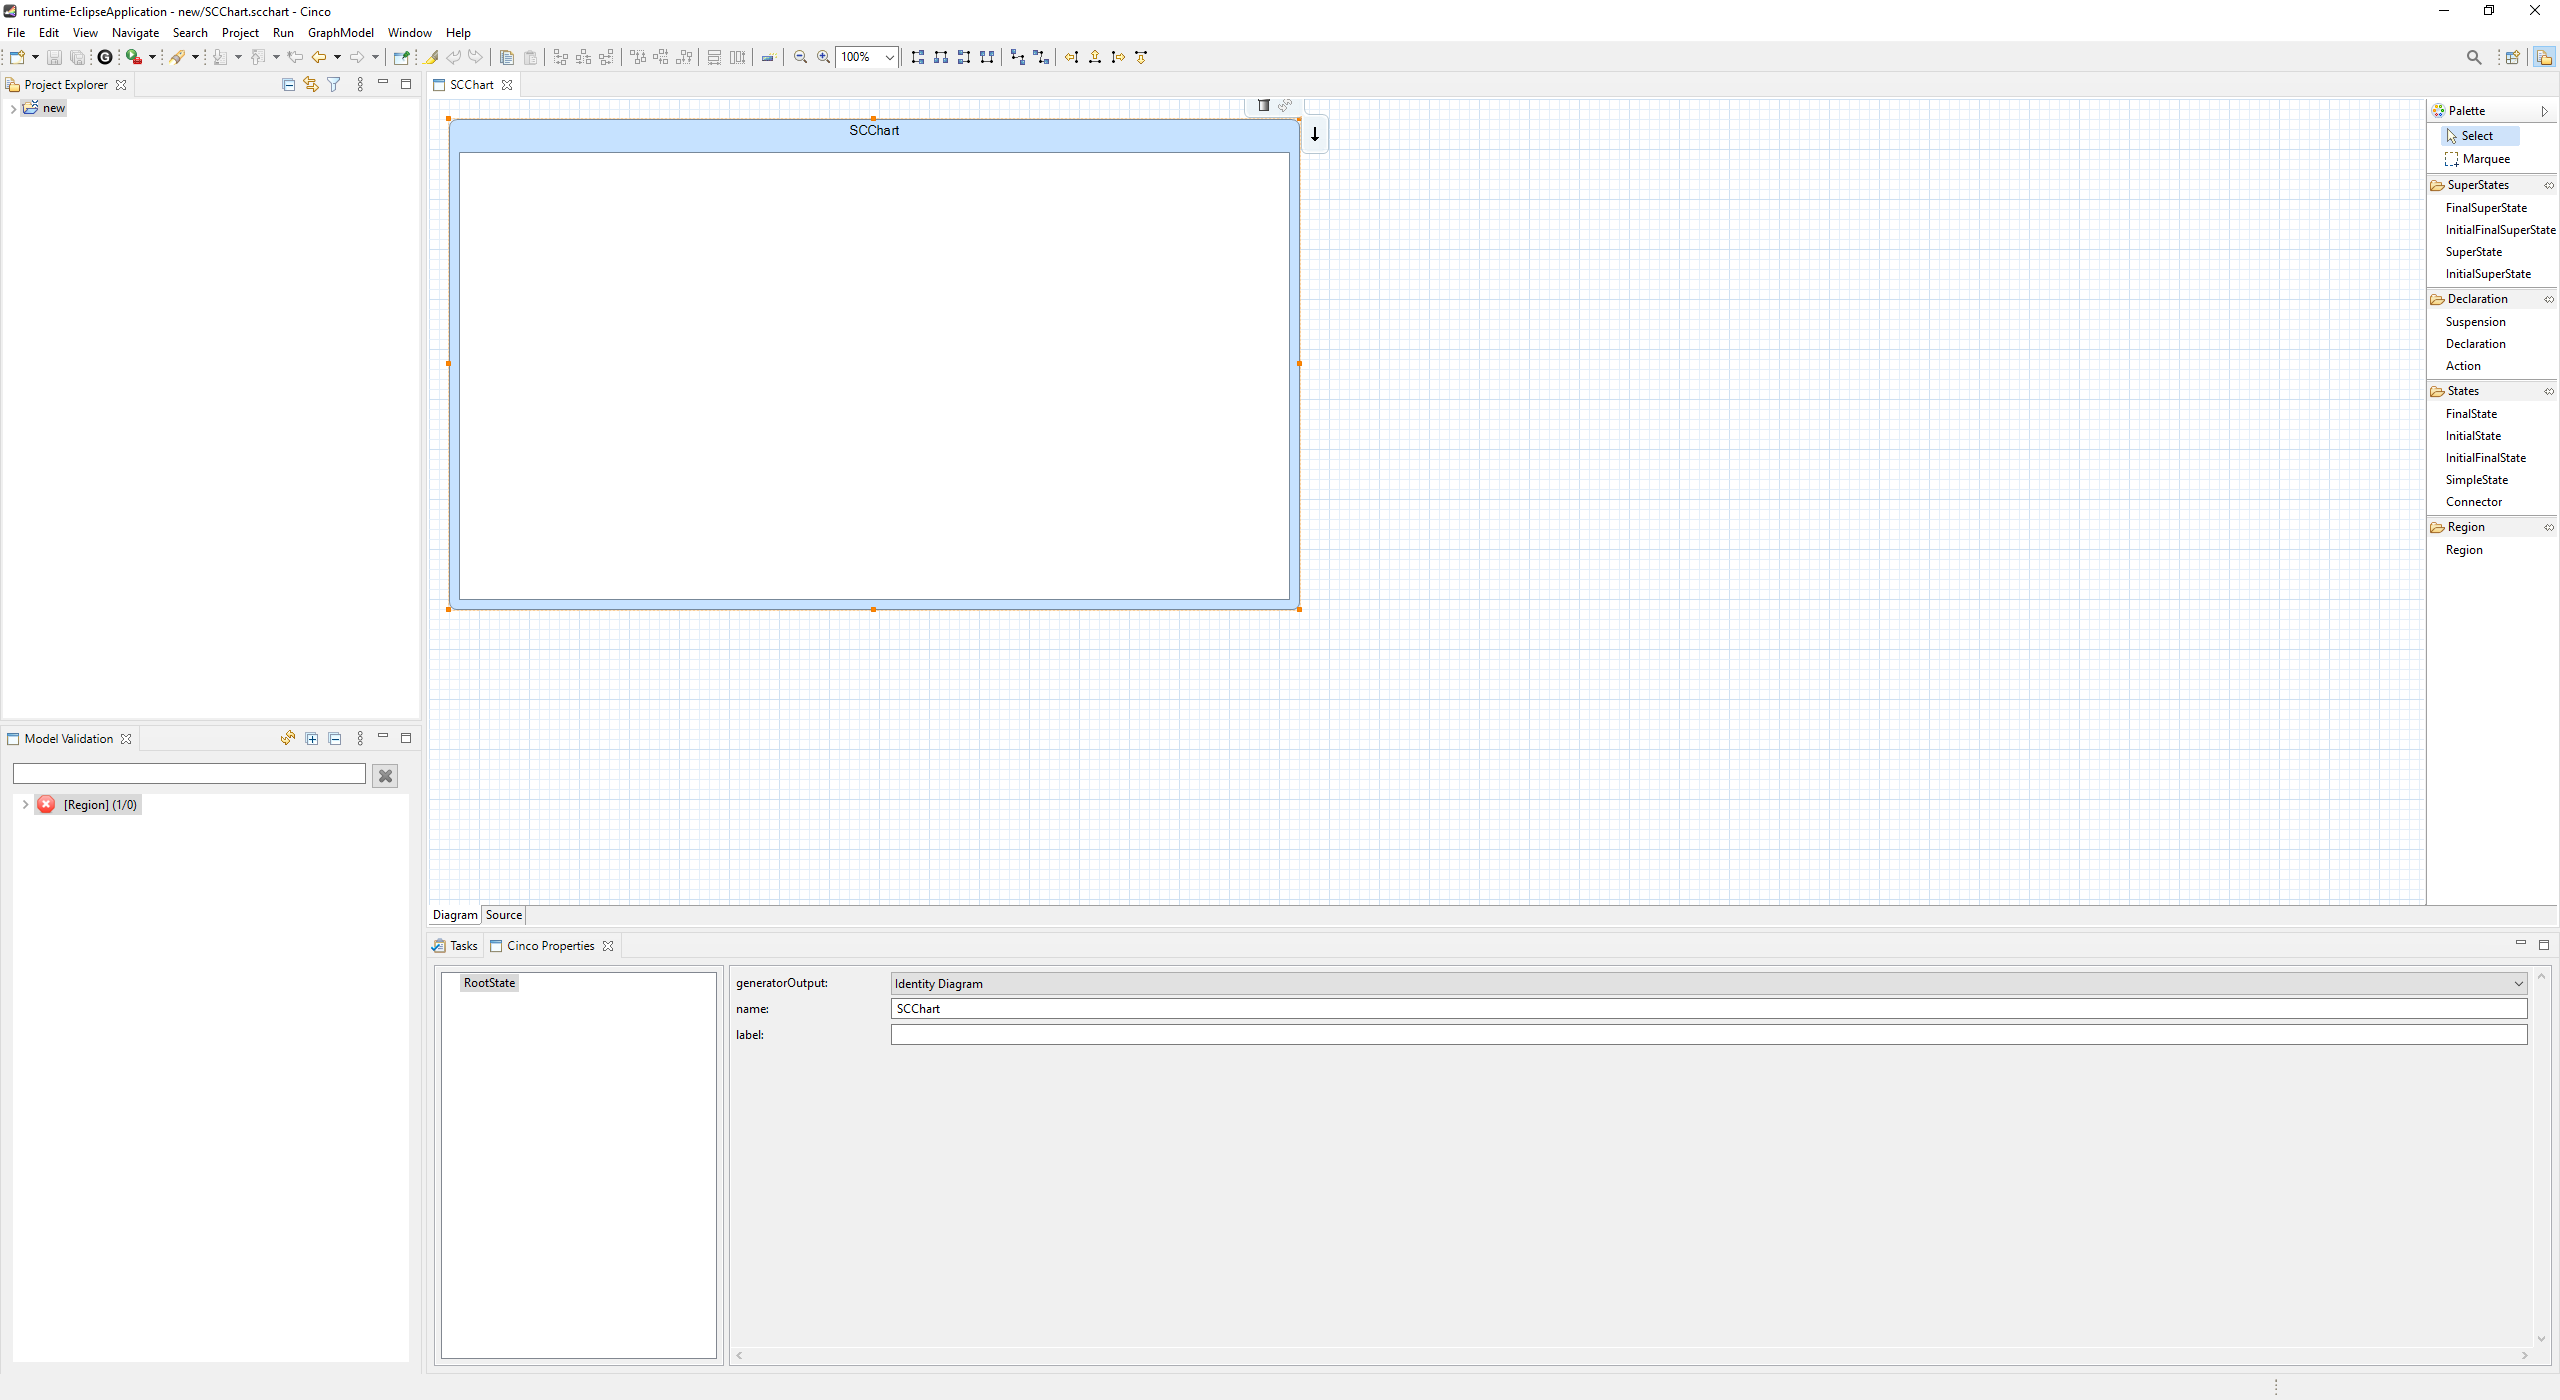
\includegraphics[width=1.0\textwidth]{bilder/User_Interface.png}
\caption{User Interface of the created SCChart Editor}
\label{fig:User_Interface}
\end{figure} 

\subsection{Visual Syntax Evaluation}

In Fig. \ref{fig:SCChartOverview_Comparison}, the upper part shows the SCCharts Overview image of Sect. \ref{Sequentially_Constructive_Statecharts} but without labels. Almost all the features of SCCharts can be seen in this picture. Below that is an SCCharts model created using the editor developed in this bachelor thesis, with a design similar to the \textit{SCCharts\_Overview} image. It can be clearly seen that these are almost identical models. Only the host code, which is declared last in fourth place in the root state in the original SCChart, is missing in the lower SCChart model. In addition, the priorities are indicated for components with only one outgoing transition, while these are not shown in the original SCChart. With deferred history transitions, the red circle of deferred is covered by the black circle of history. This is because only relative values can be assigned to the decorators and therefore no fixed distance to the end of the arrow is possible. In addition, the Appearance Provider plug-in changes the entire appearance in the style so that, for example, the line of the green triangle is also dashed for the termination transition. Nevertheless, these are only minor deviations. All in all, the components of SCCharts are clearly recognisable.

\begin{figure}[h!]
\centering
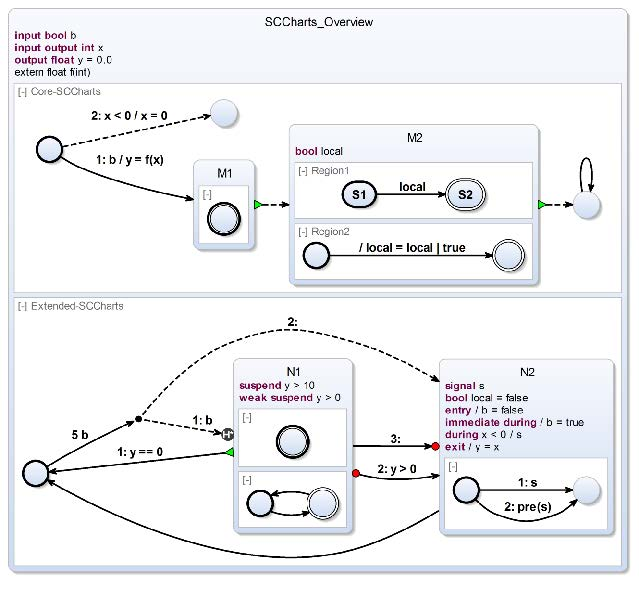
\includegraphics[width=0.9\textwidth]{bilder/SCCharts_Overview_Without_Declarations.jpg}
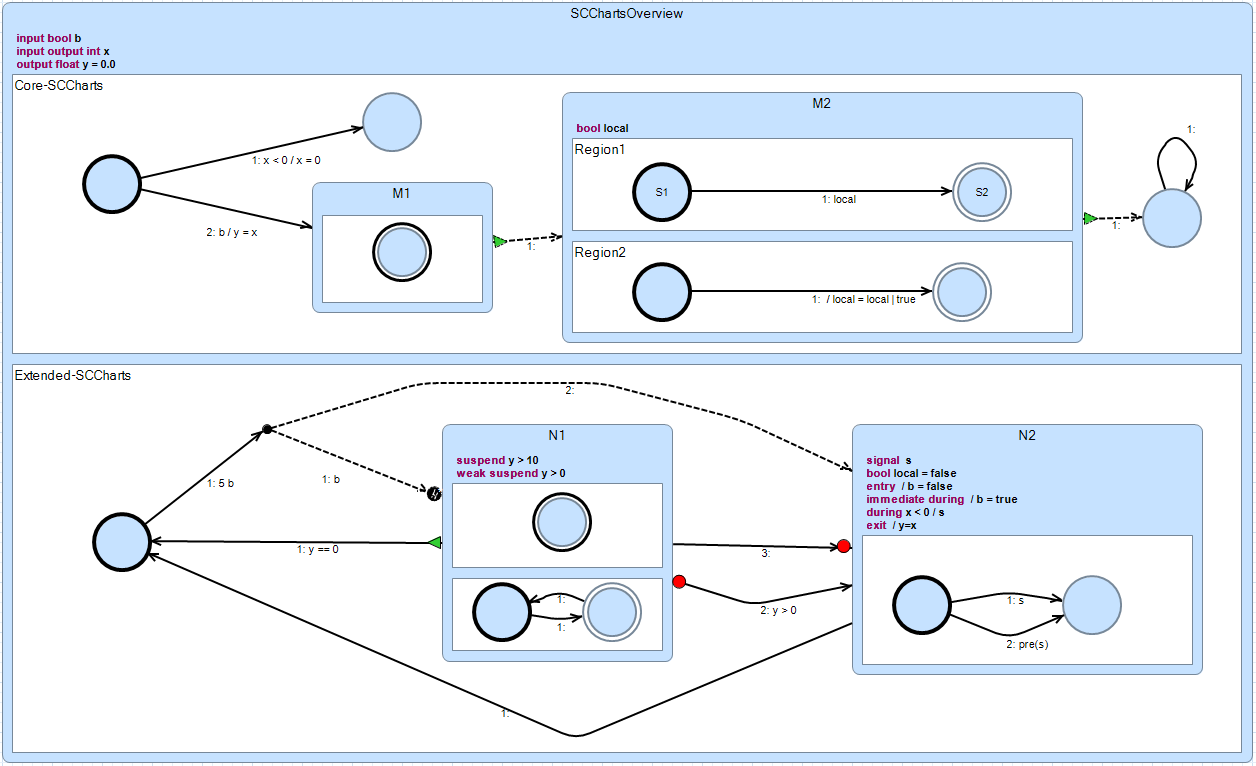
\includegraphics[width=0.9\textwidth]{bilder/CincoSCChartOverview.png}
\caption{Original SCCharts model (top) and editor SCChart model (bottom)}
\label{fig:SCChartOverview_Comparison}
\end{figure} 

\subsection{Validation Evaluation}

A validation was implemented via the MCaM plugin, which performs checks after saving the model. For a better overview and easier extension, a separate check class was created for each class or superclass of components of the MGL. Several validation functions are implemented.

Fig. \ref{fig:ValidationExample} shows some examples of validation functions. In the middle is a model with incorrect syntax. The validations are shown at the bottom left. The first error indicates that the order of outgoing transitions from an initial state, state A, is not valid. This is because both transitions originating from A have priority 1. Next, it indicates that a region does not contain exactly one initial state. This is the case in the second region of the superstate. And the last error message displayed is that for a transition, source and target are not in the same region, which is the transition from A to B. 
\begin{figure}[h!]
\centering
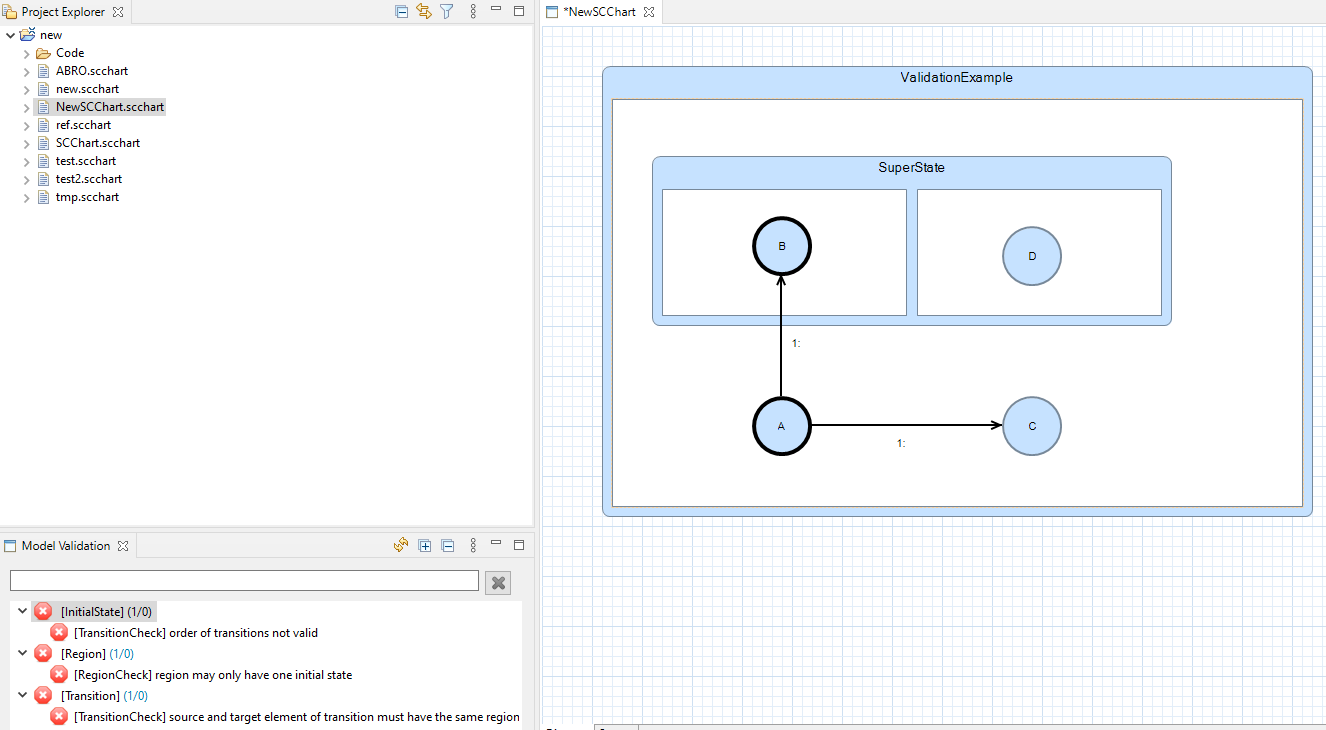
\includegraphics[width=1.0\textwidth]{bilder/CincoValidationExample.png}
\caption{Example for MCaM plugin for SCChart Validation}
\label{fig:ValidationExample}
\end{figure} 

\subsection{Code Generator Evaluation}

Through \textsc{Cinco}'s code generator meta plugin it is possible to start the code generation by clicking the generate button in the user interface. This translates the currently opened model into SCT and saves it in a file in the workspace. In addition, the KIELER SCCharts CLI is started via the command line. This takes the file in SCT format as input, and a parameter selected by the user via the root state that defines the target language of the output. This can be C or Java code, but also a SCChart diagram, which provides the possibility to compare the with the editor created SCChart model with that one of the KIELER SCChart CLI. In this way, the created model can be checked again to make sure that it meets the original requirements. In the context of this bachelor thesis, this is mainly useful to check if the code generator interprets the components of the model correctly.

An example of the output of the implemented code generator is presented in Fig. \ref{fig:CINCO_CodeGenerator}. It shows the ABRO SCChart, the "hello world" of synchronous programming~\cite{Hanxleden.2014}. Here are the functions of concurrency and preemption illustrated in a compact example. At the top left is the SCChart model from the developed \textsc{Cinco} SCChart Editor. The input and output booleans are listed in the upper section of ABRO. The strong abort transition of ABO leads to the fact that if input R is true, ABO is immediately reset, the preempt function. Within ABO, another initial superstate with 2 regions to represent concurrency, is shown. The diagram of the KIELER SCCharts CLI (bottom right) can be seen as relatively identical, as the components only differ slightly by position. This means that both the SCT code (top right) and the Java code (bottom left) created from the model (top left) with the code generator of the \textsc{Cinco} SCChart editor can be considered correct. 

However, if the model created with the SCChart editor is incorrect, the code generator also creates an incorrect SCT file, which cannot be processed by the KIELER SCCharts CLI, so that neither Java or C code nor a diagram is generated. This can also happen if, for example, a variable is specified in a condition that does not exist in the model. This allows the tool to be improved in one or two places. Nevertheless, the code generator already works quite reliably.
\begin{figure}[h!]
\centering
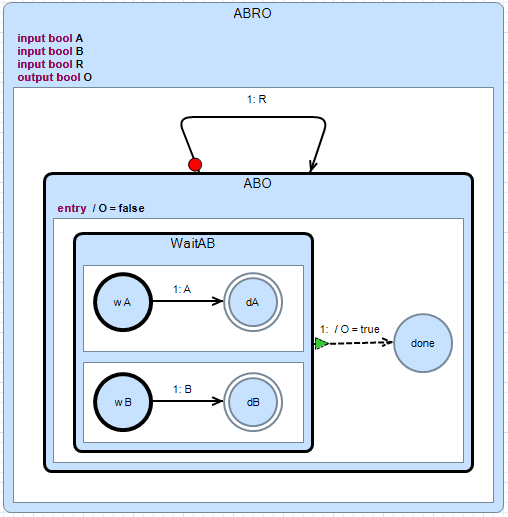
\includegraphics[width=0.5\textwidth]{bilder/CincoABROModel.png}
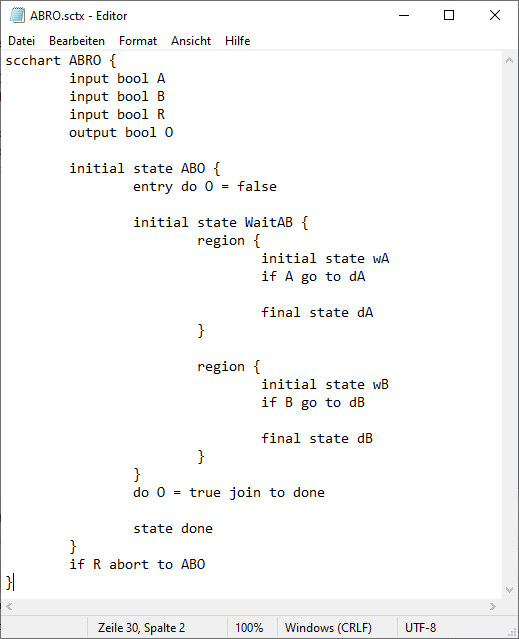
\includegraphics[width=0.43\textwidth]{bilder/ABRO_SCT.png}
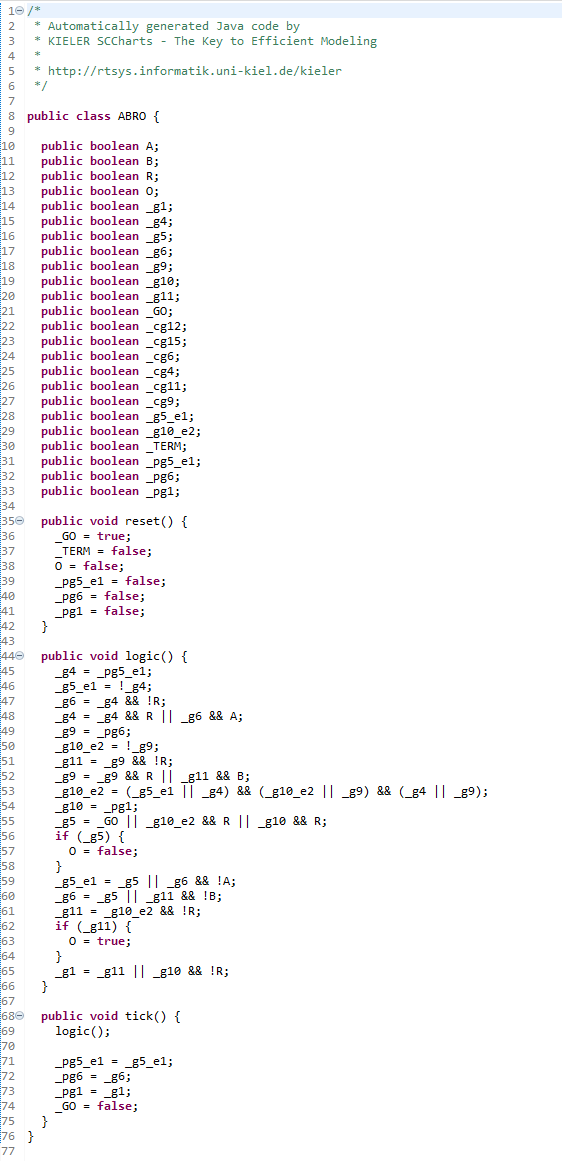
\includegraphics[width=0.35\textwidth]{bilder/ABROJavaCode.png}
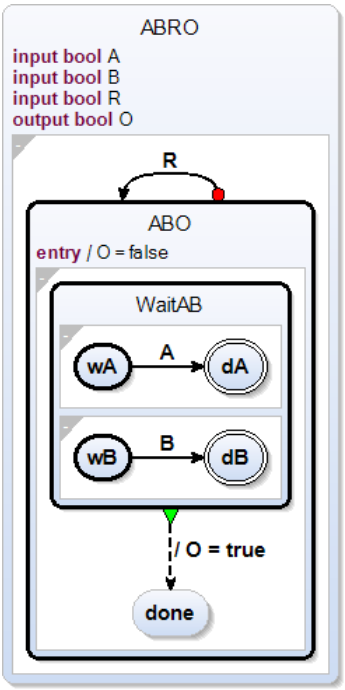
\includegraphics[width=0.38\textwidth]{bilder/ABROIdentityDiagram.png}
\caption{Output of the code generator plug-in from the ABRO SCChart}
\label{fig:CINCO_CodeGenerator}
\end{figure} 
\section{Conclusion}
With the conception and implementation of a domain specific graphical tool it should be shown that its development does not have to be tedious and complex as often assumed. The Cinco meta tool was the perfect tool for this, as it can be used to create graphical DSL tools, and its main feature is its full generation from meta specifications. This means that tools generated by cinco can be executed directly without having to adapt the code as is the case with other meta tools with semi-automatic generation. In general, cinco follows a simplicity-driven approach that imposes restrictions in order to avoid complexity.

As the graphical DSL the SCCharts language was chosen, which was designed to be used as a visual modeling language for safety-critical applications. These bring with them a wide range of features, many of which were realised in the editor that was finally developed. On the basis of previously defined requirements and a data structure containing all the important components and associations of the SCChart language that should be included in the editor, the implementation of the editor's MGL was started. Through the preliminary work with the data structure, the implementation of the MGL could be completed quickly. The SGL was oriented as closely as possible to the visual syntax of SCCharts. As a result, the visual representation of components was limited to the runtime of Cinco. Since every small difference in the visual representation can almost only be implemented by defining a new component in the MGL with its own style, which meant that many transitions of SCCharts differing only slightly still had to be defined in the MGL as own component. However, the Appearance provider, which allowed a few changes to be made at runtime, reduced the number of transitions to be defined in the MGL. After MGL and SGL were implemented, SCCHart models could be created, but it was neither intuitive nor dynamic, as all lay-outing was left to the user and the interface was not very user-friendly. The various cinco meta-plugins made it easy to modify the interface of the editor and adapt it to the DSL. They also provide a large number of functions that improve the layout of the SCChart model and thus make it possible to create more dynamic and improved models. Subsequently, the generation of integrable java and c code from the models created with the Cinco SCChart editor was realised via a further plug-in from Cinco and with the help of an SCChart compiler tool. Subsequently, the generation of integrable java and c code from the models created with the Cinco SCChart editor was realised via a further plug-in from Cinco and with the help of an SCChart compiler command line interface. The evaluation of the editor has shown that although it is not yet perfect, it is already a great support for the graphical creation of SCChart models. And the code generator is already a very useful tool. 

All in all, it was shown that a powerful and useful tool for modelling DSLs can be developed with relatively little effort. In addition, the cinco meta tool has shown that it can be used both for DSLs that offer many features and for DSLs in the security-critical area.
\chapter{Summary and Outlook} \label{Conclusion}
The final chapter summarises the presented solution and gives an outlook on improvements and extensions of the SCCharts editor.

\section{Summary}
While DSLs have the potential to empower domain experts to independently create models, reducing their reliance on programmers, they are currently underutilized. This is primarily due to the perception that developing tools for such DSLs is a laborious and time-consuming process.

To challenge this assumption, this bachelor thesis presented the development of a DSL tool using \textsc{Cinco}. \textsc{Cinco} is a tool designed for creating domain-specific graphical modeling tools with a focus on full generation of this tools from high-level specifications. The development process was demonstrated using SCCharts, a visual modeling language specifically designed for specifying safety-critical reactive systems, serving as a representative of a graph-based modeling language.

The project began with the definition of requirements for the editor to be developed. Subsequently, a data structure was designed based on the SCCharts syntax, encompassing all essential attributes and associations of SCCharts components. This data structure was used for the implementation of the MGL. Subsequently, the visual representation of the components in the editor was defined with the SGL. To enhance user-friendliness, meta plugins from \textsc{Cinco} were used to improve the handling of the editor. Additionally, a code generator was implemented, making use of the KIELER Compiler CLI, allowing for the generation of Java or C code and diagrams from the created model.

The evaluation of the user interface, visual syntax, and code generator of the developed editor demonstrated that the created DSL tool is a valuable asset for SCCharts modeling. This project has shown that a functional DSL tool can be created with relative ease, disproving the notion that DSL tool development is overly complex and tedious.
\section{Outlook}

% Anhang
\appendix
% anhang.tex
\chapter{Further Information}
\lstinputlisting[frame=single,label=SCChart_MGL,caption=The SCChart MGL]{Code/SCChart.mgl}
\lstinputlisting[frame=single,label=SCChart_SGL,caption=The SCChart SGL]{Code/SCChart.style}
\lstinputlisting[frame=single,label=ActionEvent_Xtend,caption=The ActionEvent Xtend class]{Code/ActionEvent.xtend}

\lstset{literate=
  {á}{{\'a}}1 {é}{{\'e}}1 {í}{{\'i}}1 {ó}{{\'o}}1 {ú}{{\'u}}1
  {Á}{{\'A}}1 {É}{{\'E}}1 {Í}{{\'I}}1 {Ó}{{\'O}}1 {Ú}{{\'U}}1
  {à}{{\`a}}1 {è}{{\`e}}1 {ì}{{\`i}}1 {ò}{{\`o}}1 {ù}{{\`u}}1
  {À}{{\`A}}1 {È}{{\`E}}1 {Ì}{{\`I}}1 {Ò}{{\`O}}1 {Ù}{{\`U}}1
  {ä}{{\"a}}1 {ë}{{\"e}}1 {ï}{{\"i}}1 {ö}{{\"o}}1 {ü}{{\"u}}1
  {Ä}{{\"A}}1 {Ë}{{\"E}}1 {Ï}{{\"I}}1 {Ö}{{\"O}}1 {Ü}{{\"U}}1
  {â}{{\^a}}1 {ê}{{\^e}}1 {î}{{\^i}}1 {ô}{{\^o}}1 {û}{{\^u}}1
  {Â}{{\^A}}1 {Ê}{{\^E}}1 {Î}{{\^I}}1 {Ô}{{\^O}}1 {Û}{{\^U}}1
  {ã}{{\~a}}1 {ẽ}{{\~e}}1 {ĩ}{{\~i}}1 {õ}{{\~o}}1 {ũ}{{\~u}}1
  {Ã}{{\~A}}1 {Ẽ}{{\~E}}1 {Ĩ}{{\~I}}1 {Õ}{{\~O}}1 {Ũ}{{\~U}}1
  {œ}{{\oe}}1 {Œ}{{\OE}}1 {æ}{{\ae}}1 {Æ}{{\AE}}1 {ß}{{\ss}}1
  {ű}{{\H{u}}}1 {Ű}{{\H{U}}}1 {ő}{{\H{o}}}1 {Ő}{{\H{O}}}1
  {ç}{{\c c}}1 {Ç}{{\c C}}1 {ø}{{\o}}1 {Ø}{{\O}}1 {å}{{\r a}}1 {Å}{{\r A}}1
  {€}{{\euro}}1 {£}{{\pounds}}1 {«}{{\guillemotleft}}1
  {»}{{\guillemotright}}1 {ñ}{{\~n}}1 {Ñ}{{\~N}}1 {¿}{{?`}}1 {¡}{{!`}}1 
}
%\lstinputlisting[language=Xtend,frame=single,label=SCChart_Code_Gen,caption=The code generator of the SCChart Editor]{Code/CodeGenerator.xtend}
% Abbildungsverzeichnis
\listoffigures
\addcontentsline{toc}{chapter}{Abbildungsverzeichnis}
\cleardoublepage
% Algorithmenverzeichnis
\listofalgorithms
\addcontentsline{toc}{chapter}{Algorithmenverzeichnis}
\cleardoublepage
% Literaturverzeichnis
\bibliographystyle{gerplain}
\bibliography{literatur/citation}
\addcontentsline{toc}{chapter}{\bibname}
% Erklaerung
\thispagestyle{myheadings}
\markboth{}{ERKLÄRUNG}
\addcontentsline{toc}{chapter}{Erklärung}
% erklaerung.tex
\cleardoublepage
\normalsize
Hiermit versichere ich, dass ich die vorliegende Arbeit selbstständig verfasst habe und keine anderen als die angegebenen Quellen und Hilfsmittel verwendet sowie Zitate kenntlich gemacht habe.\\\\
Dortmund, den \today \\\\\\\\
Kristopher Kettler
% EOF
\cleardoublepage
\end{document}

